%%%%%%%%%%%%%%%%%%%%%%%%%%%%%%%%%%%%%%%
% MEMOIR CLASS
\documentclass[
	12pt, 
	letterpaper, 
	oneside, 
	openright, 
	onecolumn, 
	final
]{memoir}



%%%%%%%%%%%%%%%%%%%%%%%%%%%%%%%%%%%%%%%
% BIBLIOGRAPHY
\usepackage[american]{babel}
\usepackage{csquotes}
\usepackage[
backend=biber,
style=apa
]{biblatex}

\addbibresource{urban-heat.bib} 

\begin{document}

%%%%%%%%%%%%%%%%%%%%%%%%%%%%%%%%%%%%%%%
% FRONT MATTER
\begin{titlingpage}
	\begin{center}

	
\includegraphics[width=0.14\textwidth]{../format/DLSU_Logo} 
	\vspace{4ex}
	
	%\ifGrad
	%\begin{Spacing}{1.5} 
	%	{\bfseries \Large \MakeTextUppercase{\documentTitle}}
	%\end{Spacing}
	%\else
	\begin{Spacing}{1.5} 
		Projected Changes in the Urban Heat Island Effect in \\
		Select Cities of Luzon, Philippines using RegCM5 Simulations \\
%		\textbf{[draft]}
	\end{Spacing}
	%\fi
	\vfill
	
	\rule{3cm}{0.5pt}\\
	\vfill
	
	%A \documentType \\
	%Presented to the \ifGrad \else Faculty of the \fi \\
	%\ifGrad
	%Graduate School of the \\
	%\else
	%\department \\
	%\fi
	%\college \\
	%De La Salle University \\
	
	A Thesis\\
	Presented to the Faculty of the \\
	Department of Physics \\
	College of Science \\
	De La Salle University \\
	\vfill
	
	\rule{3cm}{0.5pt}\\
	\vfill
	
	In Partial Fulfillment of the\\
	Requirements for the Degree of\\
	Bachelor of Science in Physics with Specialization in Medical Instrumentation\\
	\vfill
	
	\rule{3cm}{0.5pt}\\
	\vfill
	
	by \\
	\vspace{2.5ex}
	
	%\foreach \n in {1,...,\numberOfAuthors}{
	%	\MakeTextUppercase{
	%		\documentAuthor{surname\n}}, \ \documentAuthor{firstname\n} \\
	%}
	DOMINGO, John Ericson O.
	\vspace{2.5ex}
	
	%\monthyeardate \today \\
	\today \\
\end{center}

\clearpage
\end{titlingpage}

%\ifFinished
%\chapter*{}
%{
%	\thispagestyle{empty}
%	\begin{SingleSpace}
%		\vfill
%		
%		\ifPutLineNumbers
%		\TitleGuide
%		\fi
%		
%		\vfill
%		{
%			\footnotesize
%			\begin{Spacing}{0.75}
%				\noindent \the\year \ \\
%				\noindent All Rights Reserved. 
%				No part of this publication may be reproduced, 
%				stored in an information retrieval system, or 
%				transmitted, in any form or by any means, 
%				electronic, mechanical, by photocopying, scanning, recording, or otherwise, 
%				except under the terms of the applicable law.
%			\end{Spacing}
%		}
%	\end{SingleSpace}
%}
%\cleardoublepage


\ULCornerWallPaper{1}{./format/dlsu_thesis_paper_letterhead.pdf}

\frontmatter

\begin{SingleSpace}
	\tableofcontents
	\cleardoublepage
\end{SingleSpace}

\ClearWallPaper
\includepdf[
pages=-,
addtotoc={
	1,
	chapter,
	1,
	Approval Sheet,
	sec:approval-sheet
}
]{./frontmatter/Domingo Approval Sheet}

%%%%%%%%%%%%%%%%%%%%%%%%%%%%%%%%%%%%%%%%%%%%%%%%%
	\phantomsection % for the TOC
	\addcontentsline{toc}{chapter}{%
		Approval Sheet 
	}
	{
	\thispagestyle{empty}
	
\begin{center}
	\textbf{THESIS DEFENSE APPROVAL SHEET}
\end{center}



This thesis entitled 
``Projected Changes in the Urban Heat Island Effect in Select Cities of Luzon, Philippines using RegCM5 simulations''
prepared and submitted by
John \mbox{Ericson} O. Domingo
in partial fulfillment of the requirements for the degree of  Bachelor of Science in Physics with Specialization in Medical Instrumentation
has been examined and is recommended for acceptance and approval for ORAL EXAMINATION. 

\vspace{4ex}

\begin{center}
	\rule{5cm}{.4pt}\\
	\textbf{Edgar A. Vallar, PhD} \\
	\textit{Adviser} \\
\end{center}

\vspace{3ex}
\hrule
\vspace{3ex}

\begin{center}
	\textbf{PANEL OF EXAMINERS}\\
	Approved by the Examination Panel with a grade of \rule{1cm}{.4pt}.\\

	\vspace{5ex}
	
	\rule{5cm}{.4pt}\\
	\textbf{Maria Cecilia D. Galvez, Ph.D.}\\
	\textit{Panel Chair} \\
	\vfill

	\begin{tabular}{c c c}
		\rule{5cm}{.4pt} & \hspace {10em} & \rule{5cm}{.4pt}\\
		\textbf{Floro Junior Roque} & & \textbf{Jazzie Jao}\\ 
		\textit{Panel Member} & & \textit{Panel Member} \\
	\end{tabular}
\end{center}				

\vspace{3ex}
\hrule
\vspace{3ex}

Accepted and approved in partial fulfillment of the requirements for the degree of  Bachelor of Science in Physics with Specialization in Medical Instrumentation.

\vspace{4ex}

\begin{center}
	\rule{5cm}{.4pt}\\
	\textbf{Maria Cecilia D. Galvez, Ph.D.}\\
	\textit{Chair, Physics Department} \\
	\vfill
\end{center}

		
\cleardoublepage
%%%%%%%%%%%%%%%%%%%%%%%%%%%%%%%%%%%%%%%%%%%%%%%%

\ULCornerWallPaper{1}{./format/dlsu_thesis_paper_letterhead.pdf}

\phantomsection
\addcontentsline{toc}{chapter}{Abstract}
\begin{DoubleSpace}
	\chapter*{Abstract}

Insert abstract here.

\vspace{3ex} \noindent {\itshape Index Terms}---Keywords.

%Keep your abstract short by giving the gist/nutshell of your \MakeTextLowercase{\documentType}.	 Use the following checklist questions to help you in crafting your abstract.	
%
%\begin{itemize}
%	\item[$\square$] Did you briefly state what you intend to do?  
%	\item[$\square$] Did you concisely discuss the problem statement?
%	\item[$\square$] Did you tersely mention the objectives in general terms? 
%	\item[$\square$] Did you succinctly describe the methodology for the target audience?
%	\item[$\square$] Did you strongly describe your significant results and your conclusions?
%\end{itemize}
\end{DoubleSpace}
\cleardoublepage
%\begin{DoubleSpace}
%	\chapter*{Acknowledgments}
%		I would like to thank my regular D\&D and video game friend group: Mari, AJ, Cole, Denzel, 

I would like to thank the friends I've met during the Taiwan International Internship Program: Greg, Cydee, Glen, Aaron, Alecx, and Janica. 
%		\cleardoublepage
%\end{DoubleSpace}

%\pagenumbering{roman}

\ClearWallPaper

\includepdf[
pages=-,
addtotoc={
	1,
	chapter,
	1,
	General Research Ethics Checklist,
	sec:ethics-checklist
}
]{./frontmatter/domingo-ethics-checklist}

\includepdf[
pages=-,
addtotoc={
	1,
	chapter,
	1,
	Application for Ethics Review,
	sec:ethics-application
}
]{./frontmatter/RERC Form 6A.pdf}

\includepdf[
pages=-,
addtotoc={
	1,
	chapter,
	1,
	Certificate of Exemption,
	sec:ethics-application
}
]{./frontmatter/Certificate of Exemption.pdf}

%\includepdf[
%	pages=-,
%	addtotoc={
	%		1,
	%		chapter,
	%		1,
	%		Research Ethics Clearance Form,
	%		sec:ethics-clearance
	%	}
%]{./frontmatter/domingo-ethics-clearance}

\includepdf[
pages=-,
addtotoc={
	1,
	chapter,
	1,
	Agreement on Intellectual Property Right,
	sec:intellectual-property
}
]{./frontmatter/domingo-IP}


\includepdf[
pages=-,
addtotoc={
	1,
	chapter,
	1,
	Agreement on Intellectual Property Right,
	sec:intellectual-property
}
]{./frontmatter/domingo-IP}

\ULCornerWallPaper{1}{./format/dlsu_thesis_paper_letterhead.pdf}

\begin{SingleSpace}	
	\listoffigures
	\cleardoublepage
	
	\listoftables
	\cleardoublepage

\end{SingleSpace}
%%%%%%%%%%%%%%%%%%%%%%%%%%%%%%%%%%%%%%%
% BODY

\DoubleSpacing
%\pagenumbering{arabic}
\mainmatter

\chapter{Introduction}
\Mprintcontents
	\label{ch:intro}
	\section{Background of the Study}

\section{Significance of the Study}
	The United Nations Sustainability Goals blah blah blah.
	
	This study is also an opportunity to try newest version of the regional climate model: RegCM5. RegCM5 is blah blah blah.

\section{Objectives}

\section{Scope and Delimitations}
	\clearpage

\chapter{Review of Related Literature} 
\Mprintcontents
	\label{ch:rrl} 
	\section{Overview on Urban Heat}
	One of the United Nations’ ``17 Sustainable Development Goals'' is Sustainable Development Goal 11 (SDG 11): ``Sustainable Cities and Communities.'' 
	SDG 11 is a goal to make human settlements inclusive, safe, resilient, and sustainable (\cite{Parra2021}).
	
	In line with SDG 11, one big problem that cities are facing is the ``urban heat island.'' 
	This problem refers to the phenomenon where urban areas have higher temperatures compared to rural areas (\cite{Khan2021}).
	This problem is further exacerbated by climate change, and can cause discomfort (\cite{Bhati2018}), worsen ambient air quality, and increase morbidity and mortality (\cite {Khan2021}).
	
	
	%TODO: add information on anthropogenic heat
	%

\section{Summary of Studies on Urban Heat}	
	\subsection{North America and Europe}
		\textcite{Fallmann2016} modeled how mitigation measures for urban heat islands affected air quality in Stuttgart, Germany using WRF-Chem and a multi-layer canopy model. Findings include: 
			peak ozone concentration increasing for white roofs, 
			increase of primary pollutants due to reduced vertical mixing; and 
			decreasing average ozone concentration for urban greening and white roofs.
		
		\textcite{Karlicky2018} evaluated the impact of urban surfaces on the climate of Berlin, Munich, and Prague.
		The authors used to models: the Weather Research and Forecasting (WRF) model and Regional Climate Model (RegCM).
		An average of 2 to 3 \degree C increase in temperature due to the urban heat island effect was reported.
		They also reported that urban effects could decrease concentration of primary pollutants.
		Wind speed due to urban effects were highly dependent on the model and parametrizations used, though all of them were able to replicate the urban heat islands.
		
		\textcite{Ziter2019} evaluated the effectiveness of tree canopy cover as a mitigation strategy for urban heat.
		The authors attached sensors and a GPS device to a bike and rode around Madison, Winsconsin, USA.
		Using generalized additive models in R, they found that enough canopy cover can significantly help with cooling cities, 
			with results showing about a 1 \degree C drop in temperature.
		The researchers note that a 40\% canopy cover is needed in order to get the most cooling.
		
	\subsection{Asia}
		\textcite{Yuan2020} conducted a computational parametric study in order to evaluate the impact of urbanization in Singapore.
		Using Computational Fluid Dynamics, they examined how anthropogenic heat disperses given the city's urban morphology.
		The authors discovered that heat is hard to disperse if there is a lack of incoming wind.
		Based on the findings, the authors created a practical modeling tool in order to help with urban planning. 
		The Geographic Information System-based tool estimates how much impact anthropogenic heat has on the city's ambient temperature.
		
		\textcite{Gao2019} explored how effective different strategies are in mitigating the surface urban heat island in Wuhan China.
		Using the offline urbanized High-Resolution Land Data Assimilation System (u-HRLDAS), they showed that the best mitigation strategy for daytime urban heat islands is using green roofs and cool roofs.
		In their follow-up study (\cite{Gao2020}), the authors compared mitigation strategies in Wuhan, China to Xi'an, China.
		They found that all the mitigation strategies they considered were more effective for Xi'an than it was for Wuhan. 
		The authors explain that this is due to the differences in regional climate.
		
		\textcite{Wang2019} presented their preliminary findings on their modeling of Kuala Lumpur, Malaysia using ADMS-Urban.
		The authors verified their findings with landsat images, though their original plan was to use data from local meteorological stations.
		Wind speed depends on the time of day, but is shown to have a general inverse relationship with the intensity of the urban heat island effect.
		The study reported an urban heat island intensity of 8 \degree C.
		The study did not take into account anthropogenic heat.

	\subsection{The Philippines}
		\textcite{AlmadronesReyes2022} used remote sensing technology to examine how land use has changed in Metro Manila from 2001 to 2019. 
		They also examined the relationship between green spaces and temperature. 
		Their results show a decrease in normalized difference vegetation index, 
			as well as a 4 \degree C difference from 2001 to 2019.
		
		\textcite{Purio2022} assessed the urban heat islands in Manila City using satellite and meteorological data.
		The authors report a 6 \degree C difference between the cold and hot parts of Manila.
		In addition, they note that areas with vegetation or bodies of water have lower surface temperature compared to residential areas, roadways, and commercial buildings.
		The authors have also given six recommendations the Manila city government may use in order to mitigate urban heat.
		
		\textcite{Oliveros2019} studied a total of 19 places in the Philippines with WRF to see if their urbanization efforts have had an effect on weather.
		They noted an urban heat island effect occurring, with a reported
			0.4 \degree C to 2.4 \degree C minimum difference, and a 
			0.83 \degree C to 2.3 \degree C maximum difference
			between urban and rural areas of Metro Manila.
		They also noted that urbanization led to more rainfall, though this finding was not statistically significant.
		
		\textcite{Cortes2022} evaluated the effectiveness of urban heat mitigation strategies in Mandaue, Cebu.
		The authors used ENVI-met, a three-dimensional software model used to simulate urban areas with computational fluid dynamics.
		They found that adding more trees and using green roofs could decrease surface temperature by about 0.4 \degree C to 1.1 \degree C.
		Notably, based on the thermal comfort index, the authors concluded that people would still feel uncomfortable from the heat, despite employing mitigation strategies.

\section{Common Themes}
	Studies report a correlation between temperature and urbanization, which is to be expected.
	Reported temperature changes go from 1 \degree C (\cite{Huszar2018a}), 
		%up to 10 \degree C (\cite{Santamouris2020}).
		up to 8 \degree C (\cite{Wang2019}).
	For the Philippines specifically, reported temperature changes due to the urban heat island effect go from 0.4 \degree C (\cite{Oliveros2019}),
		up to 6 \degree C (\cite{Purio2022}).
	
	There does not seem to be one common way of simulating urban heat.
	A handful of studies use the Weather Research \& Forecasting Model (WRF) with an urban canopy model.
	Other simulations include the Regional Climate Model (RegCM),
		ADMS-Urban, 
		ENVI-met, and
		the urbanized high-resolution land data assimilation system (u-HRLDAS).
	Regardless of simulation method, the studies made sure to verify their models. For example, a handful of studies compared their simulated data to data gathered via remote sensing.
	
	There have been studies that evaluate the effectiveness of urban heat mitigation strategies outside of the Philippines, such as \textcite{Gao2019} and \textcite{Gao2020}. 
	However, there is a lack of these studies inside the Philippines.
	Out of the articles mentioned in this chapter that studied the Philippines, only \textcite{Cortes2022} directly examined the effectiveness of urban heat mitigation strategies.
	\textcite{Purio2022} gives recommendations for mitigating urban heat, but studying their effectiveness was out of the authors' scope.
	
	The majority of the articles that studied the Philippines focused on Metro Manila.
	\textcite{Cortes2022} studied Mandaue, Cebu, while \textcite{Oliveros2019} studied Tagaytay, Bulacan, and fourteen other rural areas outside Metro Manila.
	
		
	%technique, results,
		%ano basehan na may urban heat problem?
		%paano sinusukat ang basehan na yun?
		%why select this location?
		%representative ba siya?
		%areas
			%materials used in buildings, its climate, what's in the area (mostly bahay? mostly trees? tubig?)
	%theory part: the physics!
		%equations
		%what simulation
	%method
		%analytical data used
	%resap2: theory. resap3: method (together with budget gant chart intro).
	%BFAR DENR DOST-SEI
	%urban heat isalands
	%yung magpappatagaL: YUNG mga runs!
	\clearpage

\chapter{Theoretical Framework} 
\Mprintcontents
	\label{ch:theory} 
	\section{Categories of Urban Heat Island}
	
	There are two types of urban heat island based on how they are formed and how high they reach:
	surface urban heat islands and atmospheric urban heat islands (Figure \ref{fig:urban-heat-types}).
	
	\begin{figure}
		\centering
		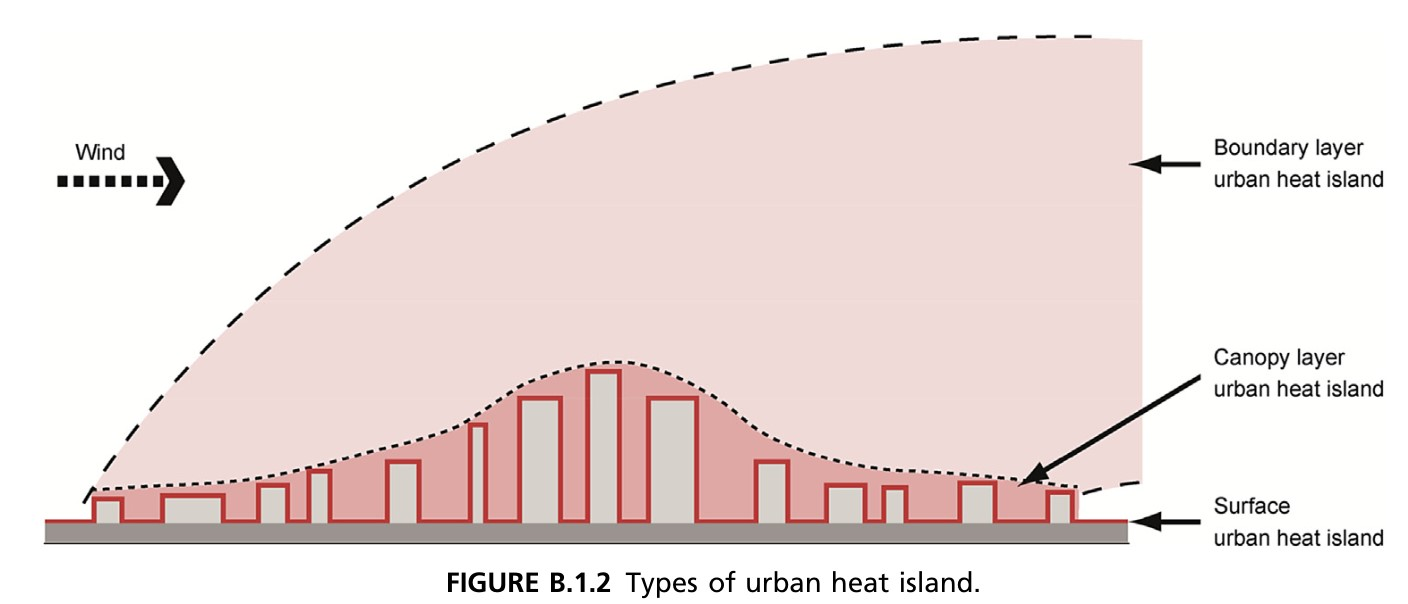
\includegraphics[width=\textwidth]{urban-heat-types}
		\caption{Types of urban heat island. Taken from \textcite{Khan2021}.}
		\label{fig:urban-heat-types}
	\end{figure}
	
	Surface urban heat islands refer to the warmer surface of urbanized areas compared to the temperature of rural surfaces, and is primarily measured by satellite thermal remote sensing data (\cite{Zhou2018}). 
	How hot a surface can reach depends on its properties.
	Dry and exposed surfaces such as roofs and pavements can become significantly hotter than the air, while shaded and moist surfaces remain as hot as the air (\cite{Khan2021}). 
	
	Atmospheric urban heat islands refer to the warmer air temperature of urbanized areas compared to the air temperature of rural areas.
	This category of urban heat island is subdivided into two more classifications:
	the canopy layer and the boundary layer (\cite{Zhou2018}).
	The canopy layer starts from the ground up to the treetops and rooftops, 
	while the boundary starts from the treetops and rooftops and extends up until point where the urban area does not affect the atmosphere (\cite{Khan2021}).
	Canopy temperatures are typically measured by sensors from meteorological stations or vehicles,
	while boundary temperatures are measured by sensors from specialized platforms such as tall towers or aircrafts (\cite{Zhou2018}).

\section{Radiant Heat and Energy Balance}
	The heating of the Earth is caused by the exchange of energy between the Sun, the Earth's atmosphere, and the Earth's surface.
	The solar rays incident on the Earth, combined with the Earth's rotation, creates a diurnal energy balance.
	These energy exchanges can be associated with an energy flux density, with units $\si{W.m^{-2}}$.
	
	\begin{figure}	
		\centering
		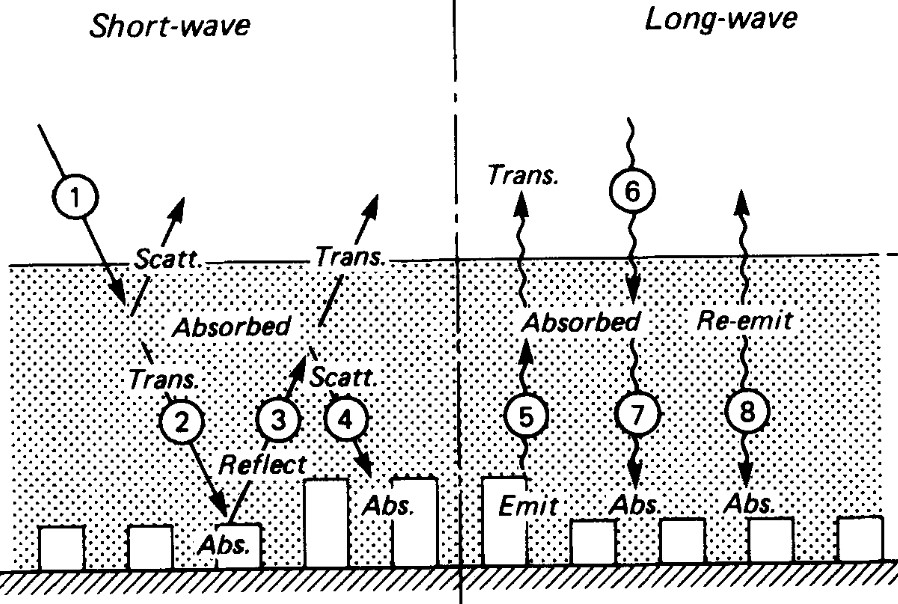
\includegraphics{radiation-budget}
		\caption{Radiation budget. Taken from \textcite{Oke1982}.}
		\label{fig:radiation-budget}
	\end{figure}

	Figure \ref{fig:radiation-budget} depicts a schematic of the fluxes present in the heating of the Earth.
	Shortwave radiation from the sun enters the urban boundary layer.
	Some of the radiation reach the surface with flux magnitude $Q_{S\downarrow}$.
	The other radiation is reflected or scattered back upward with flux magnitude $Q_{S\uparrow}$.
	The atmosphere emits longwave radiation, with some
	reaching the Earth’s surface with flux magnitude $Q_{L\downarrow}$.
	The Earth’s surface also emits longwave radiation upward with flux magnitude $Q_{L\uparrow}$. 
	The net radiation flux $Q^*$ then is given by
	\begin{equation}
		Q^* = Q_{S\downarrow} - Q_{S\uparrow} + Q_{L\downarrow} - Q_{L\uparrow}.
	\end{equation}
		
	In a rural environment, the surplus of energy provided by $Q^*$ is shared by the soil and the air.
	Heat is dissipated via conduction to the soil with flux $Q_G$,
		and via convection of sensible and latent heat with fluxes $Q_H$ and $Q_E$ respectively. 
	Thus,
	\begin{equation}
		Q^* = Q_G + Q_H + Q_E.
	\end{equation}
	An urban environment, however, modifies the energy balance in multiple ways:
	\begin{enumerate}
		\item \textbf{Canyon geometry of buildings.}
		Dense tall buildings create a canyon geometry,
			which causes radiation to get trapped in between the vertical surfaces through multiple reflections.
		This gives a greater absorption of shortwave radiation.
		This also causes a reduction of wind speed, which trap warm air.
		
		\item \textbf{Construction materials.}
		Buildings and paved surfaces are made with materials that have great heat absorption and heat storage.
		
		\item \textbf{Removal of plants and soil.}
		The replacement of plants and moist soil with paved and waterproof surfaces reduces evapotranspiration.
		More of the net radiation flux is thus converted into sensible heat, rather than latent heat.
		
		\item \textbf{Air pollution.}
		A polluted atmosphere has greater absorption and re-emission of radiation, thus increasing longwave radiation flux.
		
		\item \textbf{Anthropogenic heat.}
		There is a release of heat from man-made activities such as from
			the combustion of fuels in vehicles,
			industrial processes, and
			air-conditioning in rooms.
		Humans also release heat and moisture from metabolism, but is not as significant compared to the activities mentioned.
	\end{enumerate}

	Accordingly, extra terms are needed in the energy balance equation in order to account for these factors in the urban environment.
	The energy balance equation thus becomes
	\begin{equation}
		Q^* + Q_F= Q_H + Q_E + \Delta Q_S + \Delta Q_A,
	\end{equation}
	where $Q_F$ is the anthropogenic heat release flux,
	$\Delta Q_S$ is the storage heat flux,
	$\Delta Q_A$ is the net advection that lets heat go through the sides of the volume, and
	other terms as defined as before (\cite{Oke1988}).
	
\section{Measurement of Urban Heat Islands}
	There are three methods in which to study urban heat islands:
		in situ measurements,
		remote sensing observation,
		and modeling.
	In situ measurements blah blah blah.
	Remote sensing observations blah blah blah.
	Modeling use computers blah blah blah (\cite{Bahi2020}).
		

%\section{Radiative Transfer}
%
%	The sun heats up the atmosphere and surface of Earth through radiative transfer, the transfer of energy via electromagnetic radiation.
%	When radiation interacts with matter, it may either be absorbed, emitted, reflected, scattered, or simply transmitted.
%	The outcome depends on the wavelength of the radiation as well as the properties of the material interacting with the radiation.
%
%	\subsection{Reflection, Scattering, and Albedo}
%	%
%	%As solar radiation travels through the atmosphere,
%	%\blindtext
%	Energy may be returned to space through reflection or scattering.
%	
%	Albedo is defined as the ``ratio of the amount of solar radiation reflected by a surface to the amount received by it'' (\cite{Stewart2012}).
%	
%
%	\subsection{Absorption and Emission}
%	
%	\blindtext
%
%\section{Urban Heat Island}
%
%
%
%	\subsection{Factors Causing Urban Heat Islands}
%	
%	Different climatic and nonclimatic factors are responsible for causing urban heat islands.
%	\citeauthor{Bridgman1995} (\citeyear{Bridgman1995}, as cited in \cite{Khan2021}) lists five major ways in which urbanization can influence a city's climate:
%	\begin{itemize}
%		\item by replacing natural surfaces with asphalts, concrete, and glasses;
%		\item by replacing natural shape with blocky, angular, towering structures;
%		\item by releasing anthropogenic heat into the urban atmosphere;
%		\item by routing flow of surface runoff and preventing infiltration; and
%		\item by emitting pollutants into the urban atmosphere.
%	\end{itemize}
	\clearpage

\chapter{Methodology}
\Mprintcontents
	\label{ch:method}
	\section{Area of Study}
	This study will be conducted over Metro Manila, Philippines.
	Metro Manila, formally known as the National Capital Region, is the capital region of the Philippines.
	The region has a land area of 636 square kilometers	and has a population of 13 million people (\cite{PSA2021}).
	It is composed of one municipality: Pateros, and sixteen cities:
		Caloocan,
		Las Pinas,
		Makati,
		Malabon,
		Mandaluyong,
		Manila,
		Marikina,
		Muntinlupa,
		Navotas,
		Paranaque,
		Pasay,
		Pasig,
		Quezon City,
		San Juan,
		Taguig, and
		Valenzuela.
	A map of Metro Manila is seen in Figure \ref{fig:map-of-metro-manila}.
	
	\begin{figure}
		\centering
		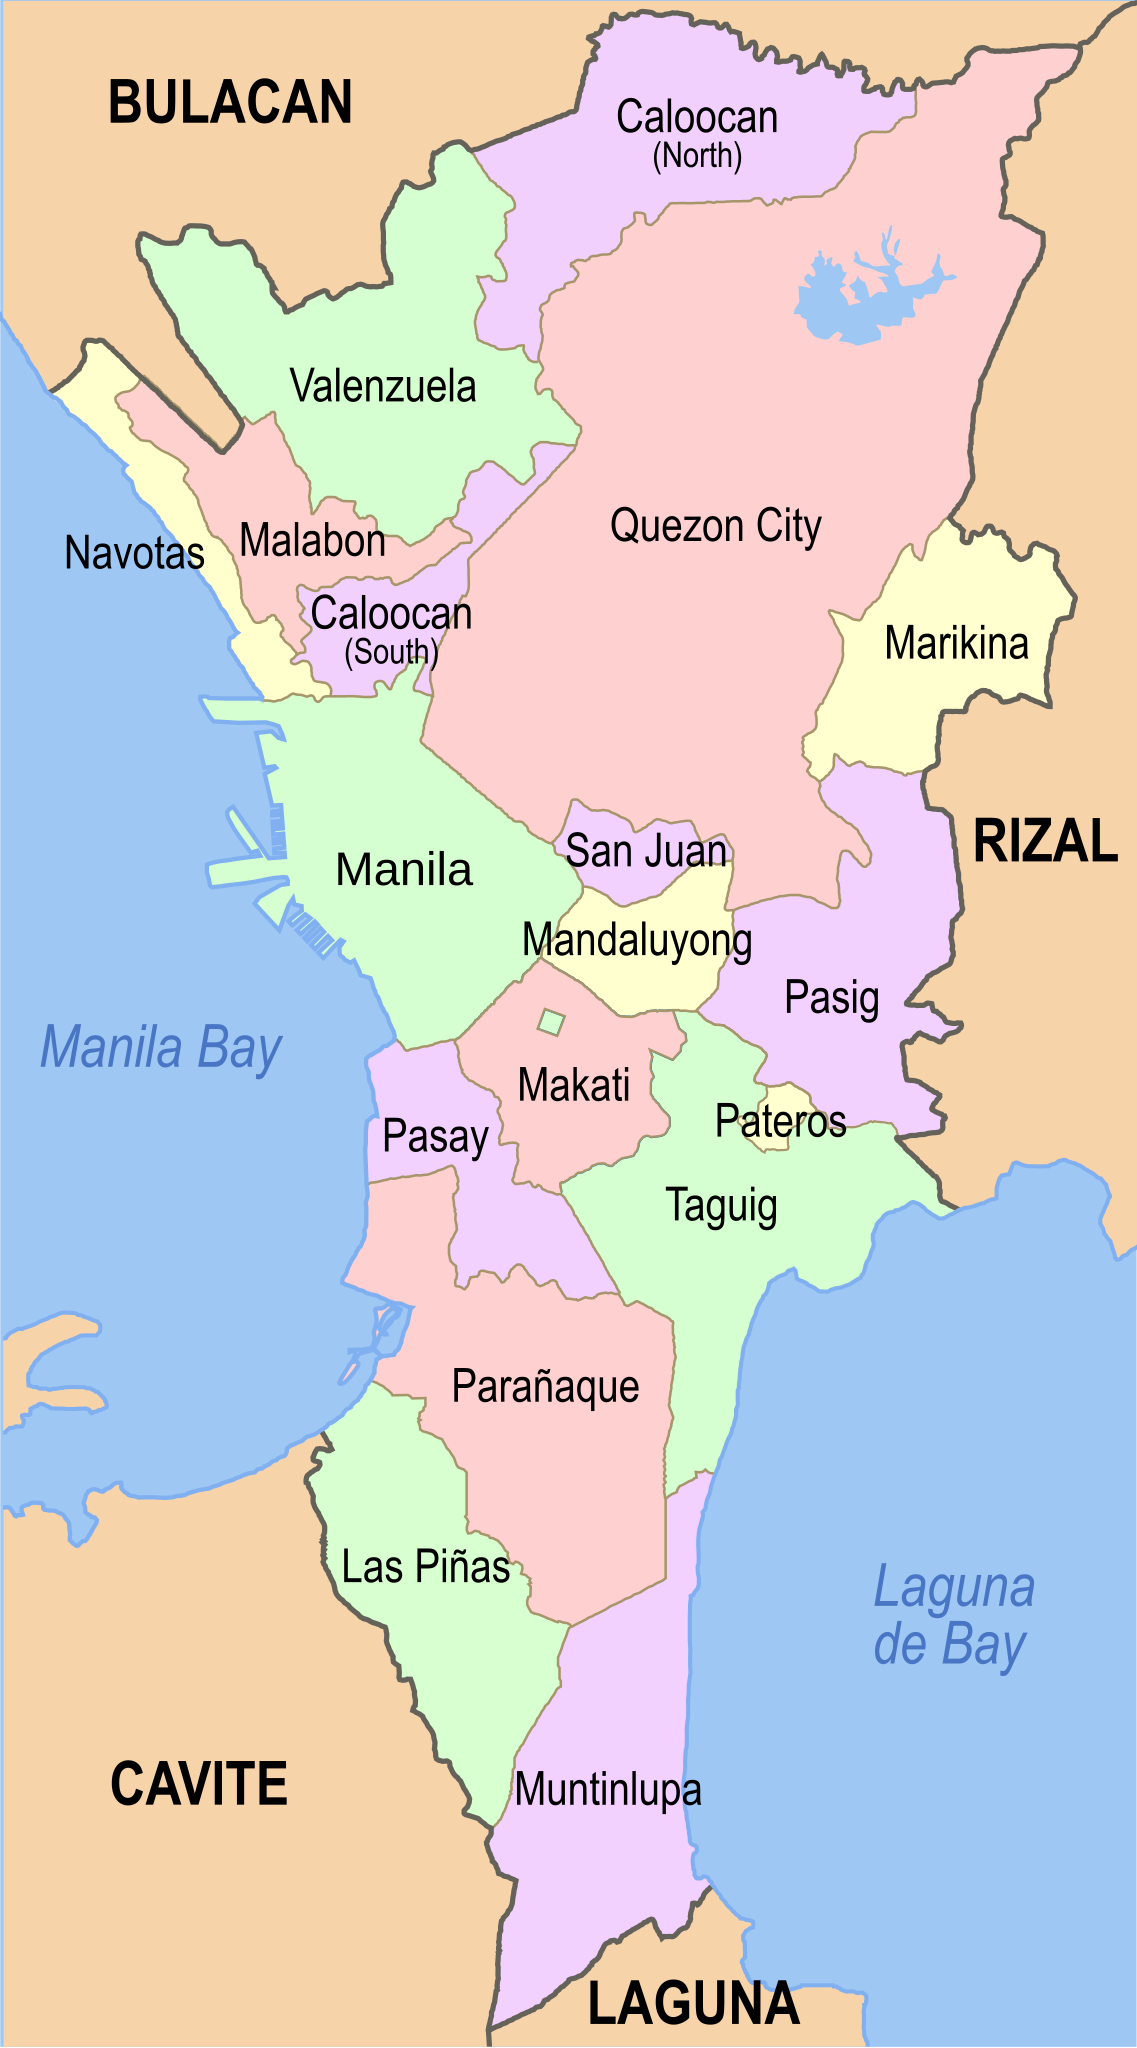
\includegraphics[width=10cm]{map-of-metro-manila}
		\caption{
			A map of Metro Manila.
			Created by Wikimedia user Philtro, and shared under a
			\href{https://creativecommons.org/licenses/by-sa/3.0/deed.en}{Creative Commons Attribution-Share Alike 3.0 Unported license}.
		}
		\label{fig:map-of-metro-manila}
	\end{figure}	
		
\section{Simulation Model}
	This study will use the latest version of the Regional Climate Model, RegCM5, which is described in detail by \textcite{Giorgi2023}.
	RegCM5 is a limited area model for long-term regional climate simulation.
	It is developed by the Abdus Salam International Centre for Theoretical Physics.
	The previous version, RegCM4, was released in 2012 (\cite{Giorgi2012}).
	
	\begin{table}	
		\caption{Configuration of the RegCM5 physics schemes.}
		\label{tab:physics-schemes}
		\centering
		\begin{tabular}{p{2 in} p{2.75 in}}
			\hline \hline
			Physics scheme & Configuration\\
			\hline
			Atmospheric radiation & Radiation scheme from the Community Climate Model version 3 (\cite{Kiehl1996}) \\
			Land surface model & Community Land Model version 4.5 (\cite{Oleson2013})\\
			Planetary boundary layer & Based on \textcite{Holtslag1990}\\
			Cumulus convection & Based on \textcite{Emanuel1991}\\
			Resolvable scale precipitation & Subgrid explicit moisture scheme (SUBEX) (\cite{Pal2000})\\
			\hline
		\end{tabular}		
	\end{table}

	This study will conduct simulations over two 20-year periods.
	The first simulation will be conducted from 2004 to 2023 to study the present.
	The results of this simulation will be compared to real meteorological data in order to determine the performance of the simulation.
	After the simulation has been evaluated to perform well, the second simulation will be run.
	The second simulation will be conducted from 2021 to 2040 to study the future.
	
	Table \ref{tab:physics-schemes} shows the physics schemes to be used in the study.
	These schemes, with the exception of the land surface model, will be used because they are the default schemes. 
	For the land surface model, the Community Land Model version 4.5 is chosen over the default, the Biosphere-Atmosphere Transfer Scheme. 
	The Community Land Model has a model for urban energy balance and climate, which the default model lacks.
	
\section{Simulation Evaluation}
	To determine the performance of the simulation, its results will be compared to real data from the Integrated Surface Database (ISD).
	The ISD is maintained by the United States National Oceanic and Atmospheric Administration, and is readily available on their website 
		(https://www.ncei.noaa.gov/products/land-based-station/integrated-surface-database).
	
	To evaluate the simulation, four performance statistics will be computed using equations \ref{eq:mean-bias} to \ref{eq:y-bar},
		where $y_i$ is the modeled value, $y_{i,\text{obs}}$ is the observed value, and $N$ is the number of data points.
	The mean bias (MB) blah blah blah.
	\begin{equation}
		\text{MB} =
			\frac{1}{N}
			\sum_{i=1}^{N}
			(y_i - y_{i,\text{obs}})
			\label{eq:mean-bias}
	\end{equation}
	The root mean square error (RMSE) blah blah blah.
	\begin{equation}
		\text{RMSE} =
			\sqrt{
				\frac{
					\sum_{i=1}^{N}
					(y_i - y_{i,\text{obs}}) ^ 2
				}{N}
			}
			\label{eq:root-mean-square-error}
	\end{equation}
	The mean absolute error (MAE) blah blah blah.
	\begin{equation}
		\text{MAE} =
			\frac{1}{N}
			\sum_{i=1}^{N} 
			|y_i - y_{i,\text{obs}}| \label{eq:mean-absolute-error}
	\end{equation}
	Lastly, the index of agreement (IOA) blah blah blah. It is computed as:
	\begin{equation}
		\text{IOA} =
			1 - 
			\frac{
				\sum_{i=1}^{N}
				(y_i - y_{i,\text{obs}}) ^ 2
			}{
				\sum_{i=1}^{N} (
					|y_i - \bar{y}| +
					|y_{i,\text{obs}} - \bar{y}|
				)^2
			}
			\label{eq:index-of-agreement}
	\end{equation}
	where
	\begin{equation}
		\bar{y} = 
			\frac{1}{N}
			\sum_{i=1}^{N} y_{i,\text{obs}}
			\label{eq:y-bar}
	\end{equation}
	The threshold for these values to determine if the model is performing well are given in Table \ref{tab:performance-statistics-threshold}, as adapted from \textcite{Bilang2022}.

	\begin{table}	
		\caption{Recommended values of statistical tests for near-surface air temperature.}
		\label{tab:performance-statistics-threshold}
		\centering
		\begin{tabular}{l l}
			\hline \hline
			Statistical parameter & Criteria\\
			\hline
			MB & $\leq \pm \qty{2.0}{\degreeCelsius}$ \\
			RMSE & $\leq \qty{3.5}{\degreeCelsius}$\\
			MAE & $\leq \pm \qty{2.0}{\degreeCelsius}$\\
			IOA	& $\geq \num{0.8}$\\
			\hline
		\end{tabular}		
	\end{table}

\section{Data Graphing and Analysis}
	The results of the simulations will be graphed.
	Data for the near-surface air temperature will be graphed as a function of time.
	This is to visually see the trend of the air temperature as time progresses.
	For the simulation of the present time, the graph of the simulation results will be overlayed on the graph of the observed data from the ISD.
	This is to visually compare the performance of the simulation with actual data.
	
	The results of the simulations will also be statistically analyzed.
	Descriptive statistics for the near-surface air temperature, such as the mean, maximum, and minimum temperature, will be computed.
	A linear regression will also be applied to see the trend at which temperature changes as time progresses.
	\stopcontents[chapters]
	\clearpage

%\chapter{Expected Results}
%	\Mprintcontents
%	\label{ch:proposal}
%	\section{Preliminary Simulations}
	In order to test if RegCM5 is working on the laboratory's workstation,
		a preliminary simulation was conducted.
	The domain of the simulation is Luzon, centered on Manila, as shown in Figure \ref{fig:proposal-domain}.
	The domain has an area of $\num{130}$ by $\num{124}$ grid cells, with a $\qty{3}{km}$ resolution.
	Data for initial and boundary condition were dated from March to September 1990,
		and the simulation itself is from March to May 1990.
	The run used 24 cores and took 14 hours to complete.
		
	\begin{figure}
		\centering
		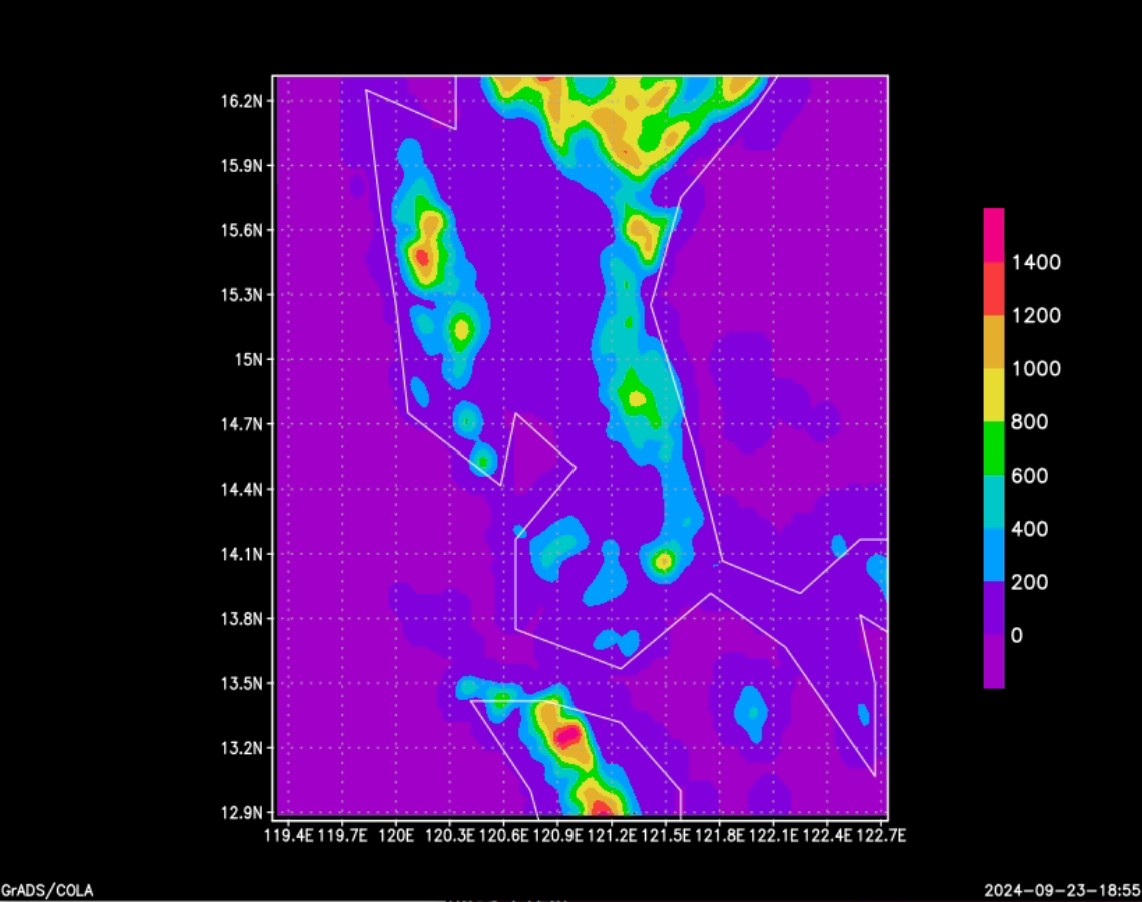
\includegraphics{proposal-domain}
		\caption{
			Surface model elevation of the domain used in the preliminary simulation.
			Domain is centered on Manila (\ang{14;35} N, \ang{121} E),
				with a grid of $\num{130}$ by $\num{124}$ cells
				and a resolution of $\qty{3}{km}$.
			Units of the elevation are in meters.
		}
		\label{fig:proposal-domain}
	\end{figure}
	
	Figure \ref{fig:proposal-manila-results} shows a comparison of the results of the simulation and the observed temperature in Manila for the month of March, 1990.
	Visually, the simulation somewhat matches the observed data, though there are large differences.
	Figures \ref{fig:proposal-naia-results} and \ref{fig:proposal-sciencegarden-results} show the same comparison as with Figure \ref{fig:proposal-manila-results}, 
		but for the Ninoy Aquino International Airport in Pasay City and the Science Garden in Quezon City, respectively.
	Visually, both cities exhibit higher simulated air temperature of around $+ \qty{2}{\degreeCelsius}$ compared to the observed data. 
	
	
	\begin{figure}
		\centering
		\begin{subfigure}{\textwidth}
			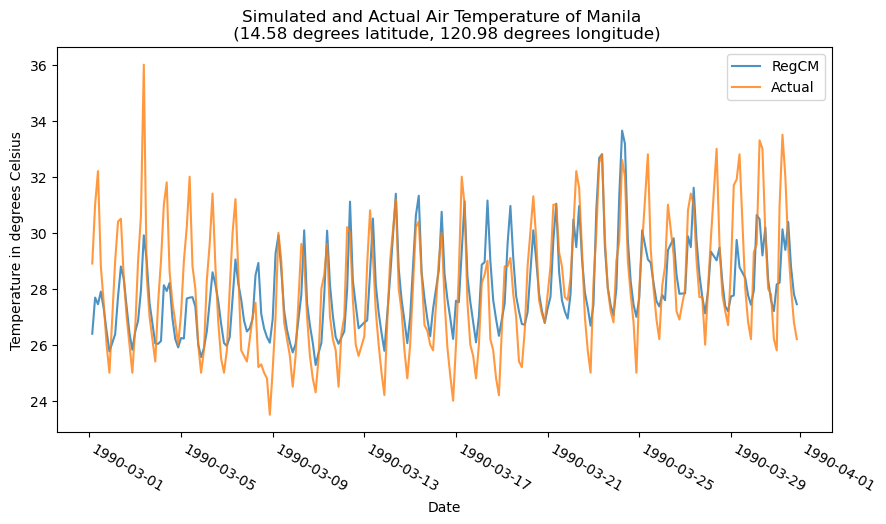
\includegraphics[width=\textwidth]{proposal-manila-both}
		\end{subfigure}
		\begin{subfigure}{\textwidth}
			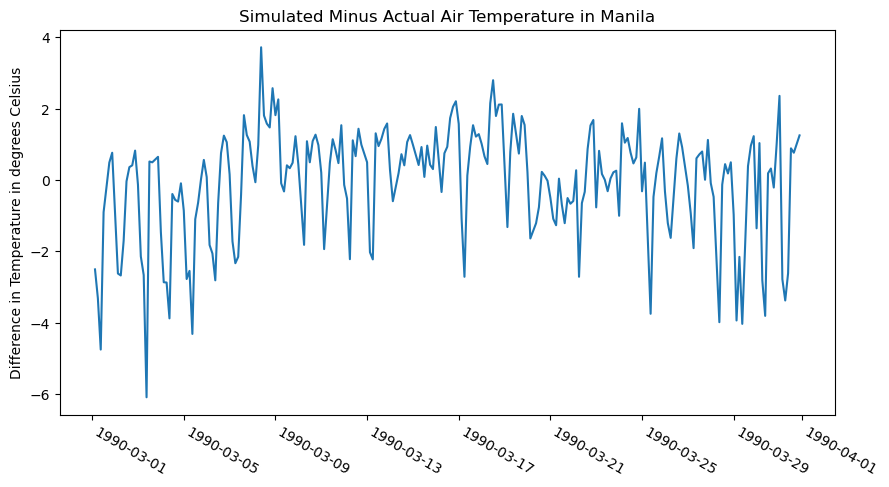
\includegraphics[width=\textwidth]{proposal-manila-difference}
		\end{subfigure}
		\caption{
			Graphs of the simulated and actual near-surface air temperature of Manila (\ang{14.58} N, \ang{120.98} E).
		}
		\label{fig:proposal-manila-results}
	\end{figure}
	
	\begin{figure}
		\centering
		\begin{subfigure}{\textwidth}
			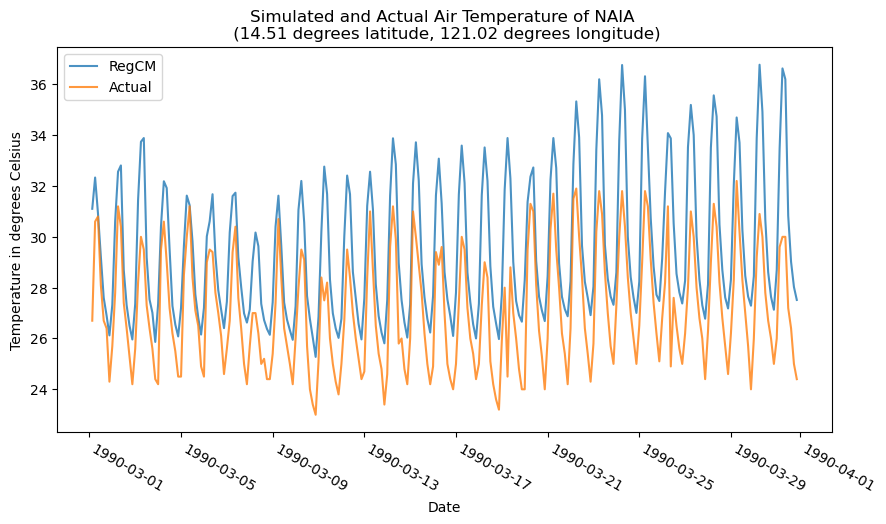
\includegraphics[width=\textwidth]{proposal-naia-both}
		\end{subfigure}
		\begin{subfigure}{\textwidth}
			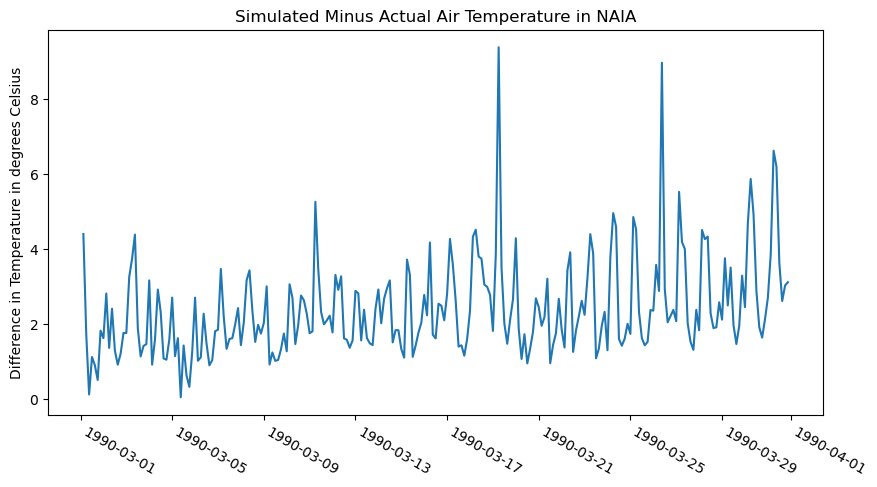
\includegraphics[width=\textwidth]{proposal-naia-difference}
		\end{subfigure}
		\caption{
			Graphs of the simulated and actual near-surface air temperature of the Ninoy Aquino International Airport, Pasay (\ang{14.51} N, \ang{120.02} E).
		}
		\label{fig:proposal-naia-results}
	\end{figure}

	\begin{figure}
		\centering
		\begin{subfigure}{\textwidth}
			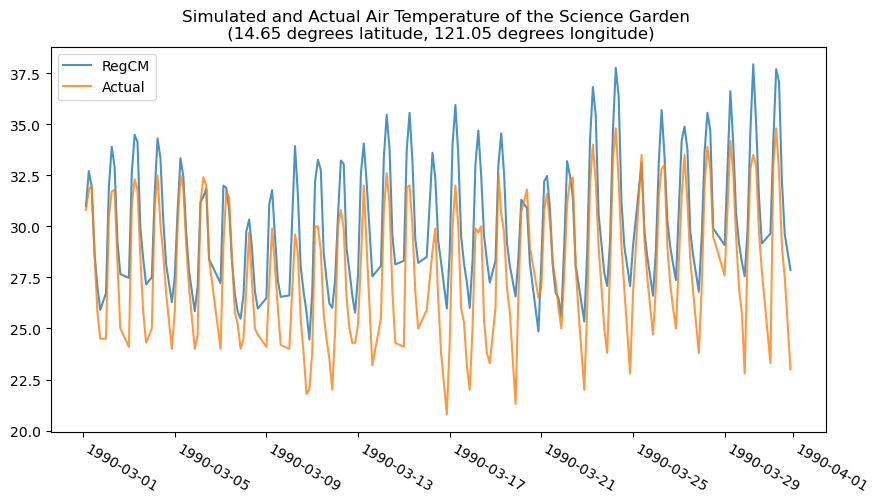
\includegraphics[width=\textwidth]{proposal-sciencegarden-both}
		\end{subfigure}
		\begin{subfigure}{\textwidth}
			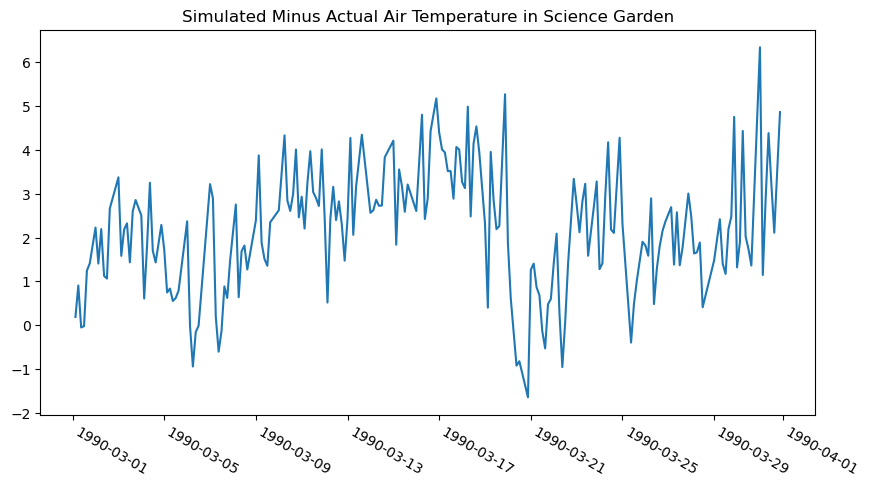
\includegraphics[width=\textwidth]{proposal-sciencegarden-difference}
		\end{subfigure}
		\caption{
			Graphs of the simulated and actual near-surface air temperature of the Science Garden, Quezon City (\ang{14.65} N, \ang{120.05} E).
		}
		\label{fig:proposal-sciencegarden-results}
	\end{figure}

\section{Budget and Timeline}

	Table \ref{tab:budget} shows the budget for this study.
	The meteorological data for the initial and boundary conditions as well as the simulation model are both free.
	They are available to download on the internet.
	The PC Workstation is available in the laboratory.
	Printing and bookbinding is estimated to be 500 Philippine Pesos,
		and will be the only cost for the study.

	\begin{table}
		\caption{Budget for this study.}
		\label{tab:budget}
		\centering
		\begin{tabular}{l r}
			\hline \hline
			Item & Price (PHP) \\
			\hline
			Meteorological data	& 0 \\
			RegCM & 0 \\
			PC Workstation & 0 \\
			Printing and bookbinding & 500 \\
			\hline
			\textbf{Total} & \textbf{500} \\
			\hline
		\end{tabular}
	\end{table}

	\begin{figure}
		\centering
		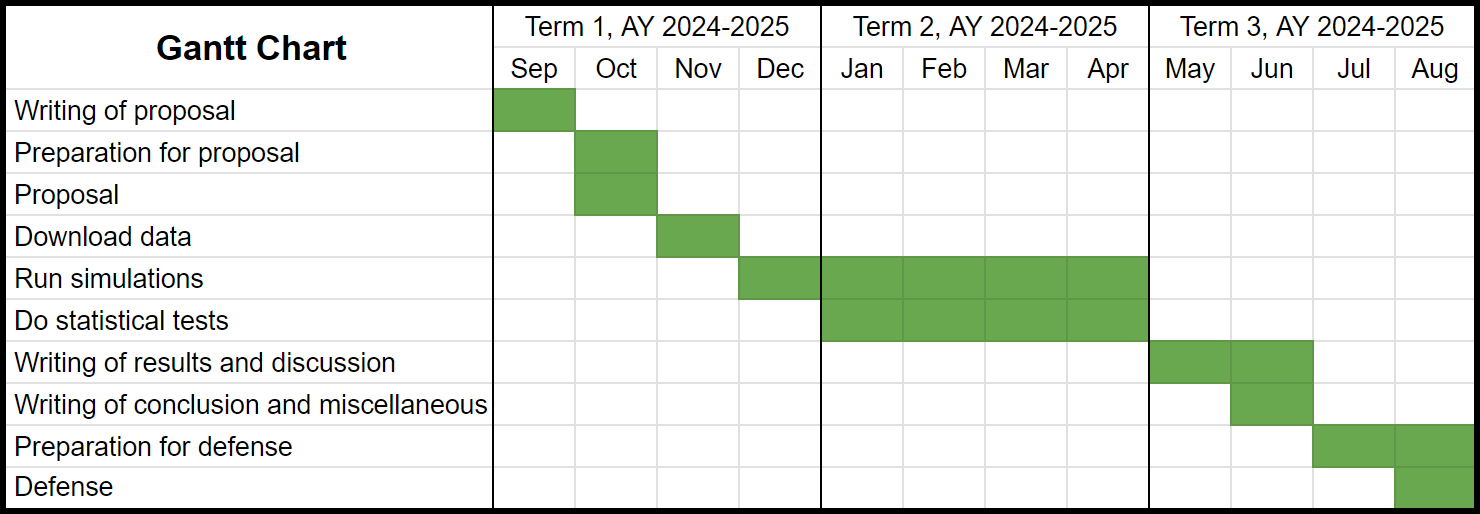
\includegraphics[width=\textwidth]{proposal-gantt-chart}
		\caption{Timeline for this study.}
		\label{fig:timeline}
	\end{figure}
%	\stopcontents[chapters]
%	\clearpage

\chapter{Results and Discussion}
	\Mprintcontents
	\label{ch:results}
	\section{Hindcast Results}
	\subsection{Model Evaluation}
		Table \ref{tab:results-evaluation-inside-mm} shows the evaluation results for the three cities inside Metro Manila: Manila, Pasay, and Quezon.
		All MB and RMSE values fall within the recommended values of $\leq \pm \qty{2.0}{\degreeCelsius}$ and $\leq \qty{3.5}{\degreeCelsius}$, respectively.
		This shows that these simulations correctly follow the average air temperature for these respective cities.
		Despite this, many runs show an IOA value $< 0.8$, indicating that these runs show bad agreement between the simulation and observed data.
		While these runs may follow the average trend for air temperature in these cities, it may not be capturing the details of how the temperature changes.
		
		\begin{table}[]
			\caption{Evaluation results for the three cities inside Metro Manila. Values that do not match the recommended values are colored in red.}
			\label{tab:results-evaluation-inside-mm}
			\centering
			\begin{tabular}{lrSSSS}
				\hline \hline
				ICBC     & \multicolumn{1}{c}{ds [\unit{km}]} & {MB [\unit{\degreeCelsius}]} & {MAE [\unit{\degreeCelsius}]}                          & {RMSE [\unit{\degreeCelsius}]} & {IOA}                               \\
				\hline
				\multicolumn{6}{c}{\textit{Manila}}                                                                                                  \\
				EIN15    & 16                          & -0.53   & 1.27                              & 1.61      & \color{red} 0.78 \\
				EIN15    & 8                           & 0.90    & 1.45                              & 1.84      & 0.85                              \\
				CNRM-CM5 & 16                          & -0.73   & 1.63                              & 2.09      & \color{red}0.57 \\
				CNRM-CM5 & 8                           & -0.38   & 1.87                              & 2.33      & \color{red}0.75 \\
				\multicolumn{6}{c}{\textit{Pasay}}                                                               \\
				EIN15    & 16                          & -0.59   & 1.24                              & 1.55      & 0.88                              \\
				EIN15    & 8                           & 0.94    & 1.40                              & 1.75      & 0.88                              \\
				CNRM-CM5 & 16                          & -0.72   & 1.87                              & 2.39      & \color{red} 0.52 \\
				CNRM-CM5 & 8                           & -0.37   & 1.78                              & 2.22      & \color{red} 0.79 \\
				\multicolumn{6}{c}{\textit{Quezon}}                                                                                  \\
				EIN15    & 16                          & -0.61   & 1.45                              & 1.81      & 0.88                              \\
				EIN15    & 8                           & 0.57    & 1.33                              & 1.70      & 0.91                              \\
				CNRM-CM5 & 16                          & -0.10   & \color{red} 2.29 & 2.77      & \color{red} 0.46 \\
				CNRM-CM5 & 8                           & -0.75   & 1.95                              & 2.44      & 0.81  \\                           
				\hline
			\end{tabular}
		\end{table}
		
		For the MAE, the CNRM-CM5 run with 16 km horizontal resolution has a value of $2.29$ in Quezon, which does not fall within the recommended value of $\leq \pm \qty{2.0}{\degreeCelsius}$.
		All other MAE values for runs in Manila, Pasay, and Quezon fall within the recommended value.
		The same run also exhibits the lowest IOA value of $0.46$, indicating that this run exhibits the poorest agreement between the simulation and observed data.
		A graph of the simulation data and observed data for Quezon using CNRM-CM5 can be seen in Figure \ref{fig:cnrm-sim-vs-observed-quezon}. 
		The simulation with the lower grid cell resolution was able to follow the average trend of the observed data, but its oscillations were much smaller than the observed data.
		The simulation with the finer resolution matches the large oscillations of the observed data more closely (Figure 2b).
		This may indicate that the high MAE is due to the failure of that run to replicate the oscillations of the observed data.
		More graphs comparing the simulated and observed data for Manila, Quezon, and Pasay are found in Appendix \ref{app:model-evaluation-graphs}.

		
		\begin{figure}	
			\centering
			\includegraphics[width = \textwidth]{CNRM 16 km/Quezon}
			\includegraphics[width = \textwidth]{CNRM 8 km/Quezon}
			\caption{
				A comparison of the simulated data (orange) and observed data (blue) in the city of Quezon using the CNRM-CM5 ICBC with 16 km resolution (above) and 8 km resolution (below).
			}
			\label{fig:cnrm-sim-vs-observed-quezon}
		\end{figure}
		
		Table \ref{tab:results-evaluation-outside-mm} shows the evaluation results for the three cities outside of Metro Manila: Baguio, Angeles, and Olongapo.
		For Baguio, three out of the four sensitivity runs performed poorly.
		The EIN15 run with 16 km resolution exhibited MB, MAE, and IOA values outside of the recommended value.
		The CNRM-CM5 run with 16 km resolution had all of its performance statistics fall outside of the recommended values, and showed the lowest IOA out of all the cities and runs.
		While the MB and RMSE of the CNRM-CM5 run with 8 km resolution are within recommended values, its MAE and IOA do not.
		Only the EIN15 run with 8 km resolution show all performance statistics within recommended values.
		A graph of the observed data and simulation data using CNRM-CM5 for Baguio is seen in Figure \ref{fig:cnrm-sim-vs-observed-baguio}.
		The lower resolution run overshoots the observed data by around $\qty{8}{\degreeCelsius}$, and exhibits smaller oscillating behavior compared to the observed data.
		The higher resolution shows a closer match to the observed data, with the simulation roughly matching the trend and oscillating behavior of the observed.
			
		\begin{table}[]
			\caption{Evaluation results for the three cities inside Metro Manila. Values that do not match the recommended values are colored in red.}
			\label{tab:results-evaluation-outside-mm}
			\centering
			\begin{tabular}{lrSSSS}
				\hline \hline
				ICBC     & \multicolumn{1}{c}{ds [\unit{km}]} & {MB [\unit{\degreeCelsius}]} & {MAE [\unit{\degreeCelsius}]}                          & {RMSE [\unit{\degreeCelsius}]} & {IOA}                               \\
				\hline
				\multicolumn{6}{c}{\textit{Baguio}}                                                                                                                                                    \\
				EIN15    & 16                          & \color{red} 2.48 & \color{red}  2.60  & 3.08                              & \color{red}  0.76  \\
				EIN15    & 8                           & 1.49                              & 1.91                              & 2.33                              & 0.84                              \\
				CNRM-CM5 & 16                          & \color{red}  8.77  & \color{red}  8.77  & \color{red}  9.10  & \color{red}  0.32  \\
				CNRM-CM5 & 8                           & 0.60                              & \color{red}  2.05  & 2.62                              & \color{red}  0.79  \\
				\multicolumn{6}{c}{\textit{Angeles}}                                                                                                                      \\
				EIN15    & 16                          & -0.48                             & 1.47                              & 1.83                              & 0.90                              \\
				EIN15    & 8                           & -0.64                             & 1.48                              & 1.87                              & 0.91                              \\
				CNRM-CM5 & 16                          & 0.41                              & \color{red}  2.42  & 2.84                              & \color{red}  0.45  \\
				CNRM-CM5 & 8                           & -1.98                             & \color{red}  2.59  & 3.13                              & \color{red}  0.76  \\
				\multicolumn{6}{c}{\textit{Olongapo}}                                                                                                                                      \\
				EIN15    & 16                          & -1.52                             & 1.80                              & 2.16                              & 0.85                              \\
				EIN15    & 8                           & -0.55                             & 1.55                              & 1.95                              & \color{red}  0.78  \\
				CNRM-CM5 & 16                          & 0.06                              & \color{red}  2.18  & 2.63                              & \color{red}  0.44  \\
				CNRM-CM5 & 8                           & -1.21                             & 1.98                              & 2.51                              & \color{red}  0.67 \\
				\hline
			\end{tabular}
		\end{table}
		
		\begin{figure}	
			\centering
			\includegraphics[width = \textwidth]{CNRM 16 km/Baguio}
			\includegraphics[width = \textwidth]{CNRM 8 km/Baguio}
			\caption{
				A comparison of the simulated data (orange) and observed data (blue) in the city of Baguio using CNRM-CM5 with 16 km resolution (above) and 8 km resolution (below).
			}
			\label{fig:cnrm-sim-vs-observed-baguio}
		\end{figure}
		
		From these results, Baguio is shown to be hard to accurately simulate.
		One reason why this may be the case is because of the topology of the city.
		Baguio's elevation is about 1,500 m above sea level, unlike the other cities which are situated near sea level.
		Furthermore, since Baguio is situated on a mountain, its nearby topology is sloped, unlike other cities where it is mostly level.
		This more complex topology may need a higher resolution in order to accurately simulate the atmospheric conditions of that region.
		
		For Angeles, the two EIN15 runs have evaluation statistics that match the recommended values.
		Furthermore, the two runs show the highest IOA values among all the runs, with a value of $0.90$ for the 16 km run and $0.91$ for the 8 km run.
		The two CNRM-CM5 runs in Angeles both have MB and RMSE values that pass the benchmark, but have MAE and IOA values that do not.
		
		For Olongapo, the two EIN15 runs both show good results among all the metrics, except for the IOA.
		The two CNRM-CM5 runs also show a low IOA, indicating inaccurate values for this station.
		
		It can be seen that in general, increasing the horizontal resolution of the simulation will increase the IOA, giving a more accurate simulation.
		One exception to this observation is for Olongapo.
		When going from a 16 km resolution to an 8 km resolution using EIN15, MB, MAE, and RMSE values improved, but the IOA worsened from $0.85$ to $0.78$.
		A graph of the observed data and simulation data using EIN15 for Olongapo is seen in Figure \ref{fig:ein15-sim-vs-observed-olongapo}.
		While the simulation using the lower resolution undershoots the observed temperature by a few degrees Celcius, the size of its oscillations closely resemble the observed data.
		The simulation using the higher resolution exhibits a smaller oscillation size compared to the observed data, though its average more closely follows the observed.
		One reason for this may be because of the station being situated by a bay.
		The nearby water can play a part with the station’s air temperature, which the simulation settings may not have accounted for.
		With the lower resolution, the interaction with water may have been negligible enough as to not affect settings, but the higher resolution gives more grid cells over water, which is perhaps why the accuracy worsened.		
		
		\begin{figure}	
			\centering
			\includegraphics[width = \textwidth]{EIN15 16 km/Olongapo}
			\includegraphics[width = \textwidth]{EIN15 8 km/Olongapo}
			\caption{
				A comparison of the simulated data (orange) and observed data (blue) in the city of Olongapo using EIN15 with 16 km resolution (above) and 8 km resolution (below).
			}
			\label{fig:ein15-sim-vs-observed-olongapo}
		\end{figure}
		
		Out of the four runs, the run using EIN15 with 8 km resolution performs the best.
		The IOA values for each station, except Olongapo, matches the recommended values of $> 0.8$.
		This means that simulations using these settings are accurate for the places studied, and can be used for future research.
		One limitation of EIN15 is that it is not compatible for forecasts, only hindcasts. Studies of future trends will need to use another ICBC such as CNRM-CM5, which is  a general climate model that does support forecasting.
		One trade-off though in using a higher horizontal resolution is that it can slow down the time it takes for the simulation to finish, as the simulation needs more grid cells.
		Also, for a given horizontal resolution, the EIN15 run performed more accurately compared to the CNRM-CM5 run. 
		This shows that runs using CNRM-CM5 need a higher horizontal resolution than EIN15 in order to exhibit the same accuracy.

	\subsection{Analysis}
		For these analyses, Olongapo is excluded from the analysis as it shown in the previous subsection to not be accurate to the observed data.
		Figure \ref{fig:hindcast-yearly-mean} shows a line graph  of the yearly mean near-surface air temperature.		
		Pasay has the highest yearly mean temperature per month, with Manila as the second highest.
		Both Pasay and Manila have almost the same mean near-surface air temperature at around $\qtyrange{29}{30}{\degreeCelsius}$, with Manila's being slightly lower than Pasay's.
		Quezon has the third highest temperature at around $\qty{28}{\degreeCelsius}$, 
			and Angeles has the fourth at around $\qtyrange{26}{27}{\degreeCelsius}$.
		Baguio has the lowest near-surface air temperature at $\qtyrange{20}{21}{\degreeCelsius}$.
		
		\begin{figure}	
			\centering
			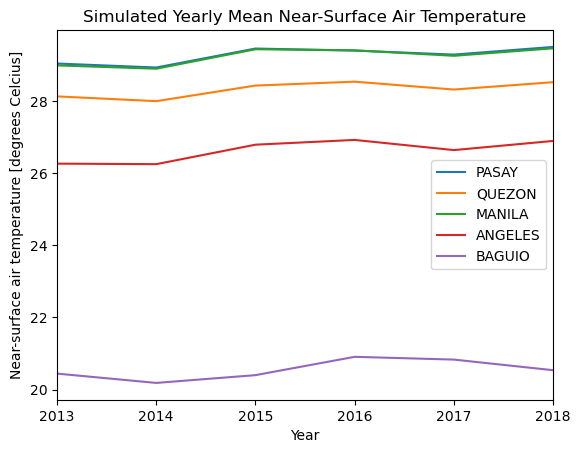
\includegraphics[width = 0.45\textwidth]{hindcast/yearly-mean}
			\caption{
				The simulated yearly mean near-surface air temperature for each of the six cities (EIN15 ICBC with 8 km horizontal resolution).
			}
			\label{fig:hindcast-yearly-mean}
		\end{figure}

		For all cities, the year 2014 has the lowest yearly mean air temperature.
		The air temperature then rises for the years 2015 and 2016,
			lowers for the year 2017,
			before rising again in the year 2018,
				except for Baguio which lowers.
		One reason for this may be because of El Niño-Southern Oscillation effects.
		The years of El Niño-Southern Oscillation effects are as follows:
			2012 to 2013 and 2013 to 2014 correspond to a neutral year,
			2014 to 2015 corresponds to a weak El Niño,
			2015 to 2016 corresponds to a very strong El Niño,
			2016 to 2017 corresponds to a weak La Niña,
			and
			2017 to 2018 also corresponds to a weak La Niña
			(\cite{Null2025}).
		Since 2016 is a year of very strong El Niño effects, the mean temperature of that year is heightened for all cities analyzed.

		\begin{figure}	
			\centering
			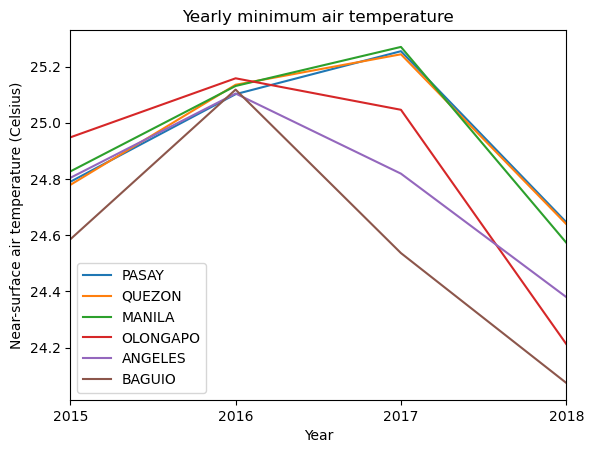
\includegraphics[width = 0.45\textwidth]{hindcast/yearly-min}
			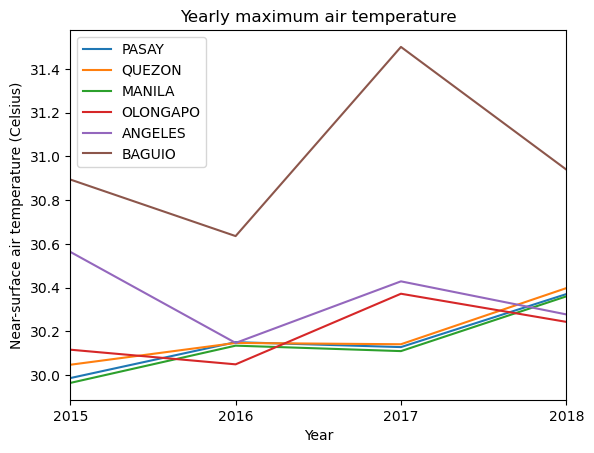
\includegraphics[width = 0.45\textwidth]{hindcast/yearly-max}
			\caption{
				The simulated yearly minimum and maximum near-surface air temperature for each of the six cities (EIN15 ICBC with 8 km horizontal resolution).
			}
			\label{fig:hindcast-yearly-min-max}
		\end{figure}
	
		Figure \ref{fig:hindcast-yearly-min-max} shows the yearly minimum and maximum near-surface air temperature for the cities.
		The maximum for all cities except Baguio can reach around $\qtyrange{37}{39}{\degreeCelsius}$ per year.
		Meanwhile, Baguio's maximum reaches around $\qty{29}{\degreeCelsius}$. 
			
		\begin{figure}	
			\centering
			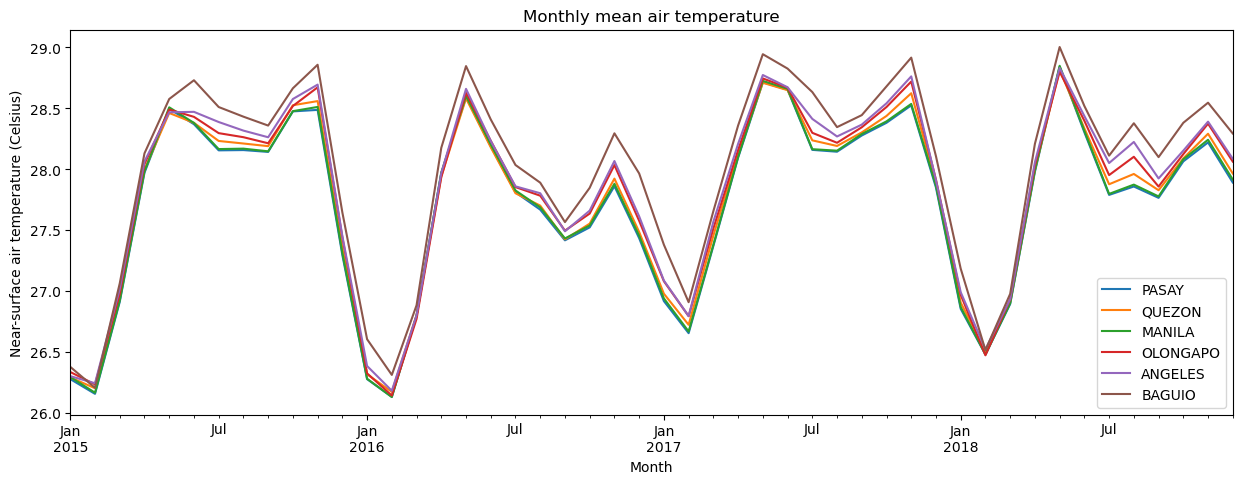
\includegraphics[width = \textwidth]{hindcast/monthly-mean}
			\caption{
				The simulated monthly mean near-surface air temperature for each of the six cities (EIN15 ICBC with 8 km horizontal resolution).
			}
			\label{fig:hindcast-monthly-mean}
		\end{figure}
	
		Figure \ref{fig:hindcast-monthly-mean} shows the simulated monthly mean near-surface air temperature.
		From the figure, February appears to be the coldest month per year.
		From then, air temperature rises until it peaks at May.
		Air temperature then lowers, during the months of July to September,
			and then rises again, peaking at November.
		It then lowers until February, and the cycle repeats for the next year.
		These results match the expected seasonal trends for air temperature in the Philippines.
		
		\begin{figure}	
			\centering
			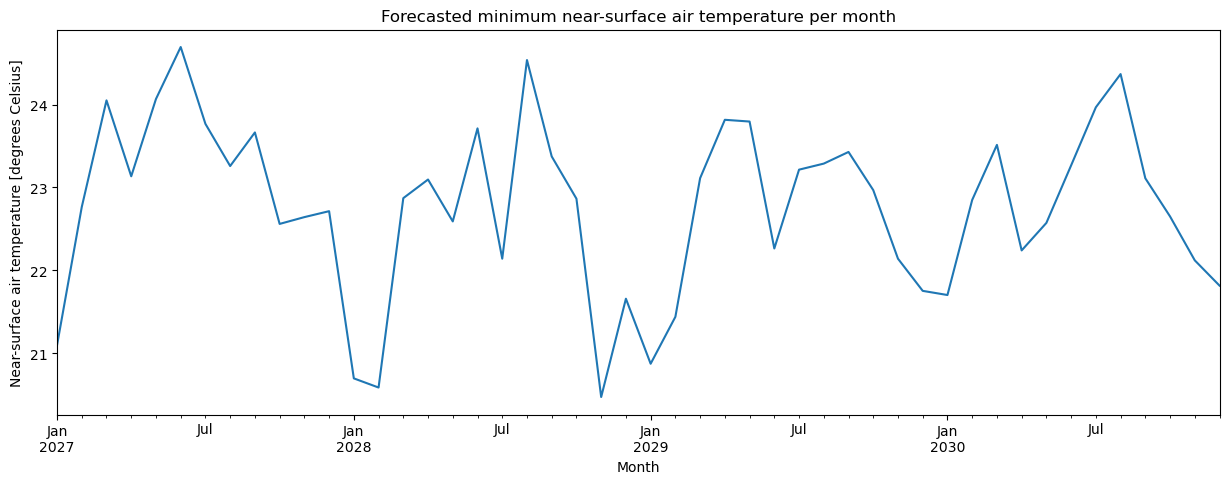
\includegraphics[width = \textwidth]{hindcast/monthly-min}
			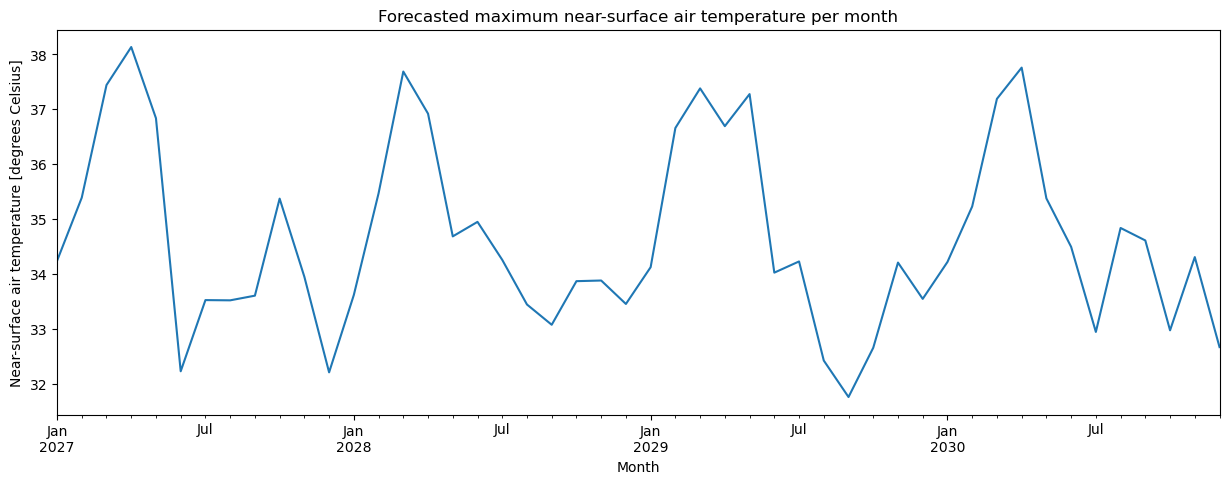
\includegraphics[width = \textwidth]{hindcast/monthly-max}
			\caption{
				The simulated monthly minimum and maximum near-surface air temperature for each of the six cities (EIN15 ICBC with 8 km horizontal resolution).
			}
			\label{fig:hindcast-monthly-min-max}
		\end{figure}

		\begin{figure}	
			\centering
			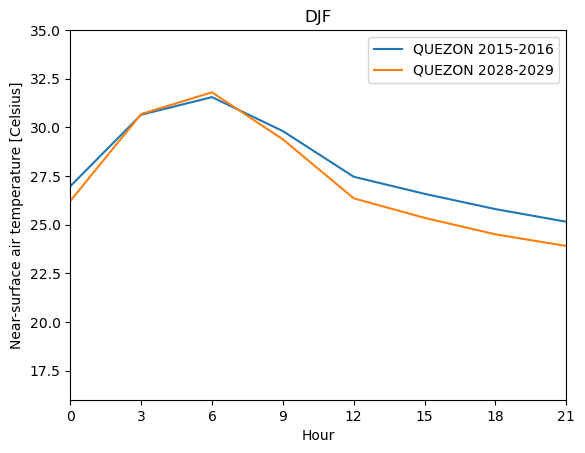
\includegraphics[width = 0.45 \textwidth]{hindcast/hourly-mean-djf}
			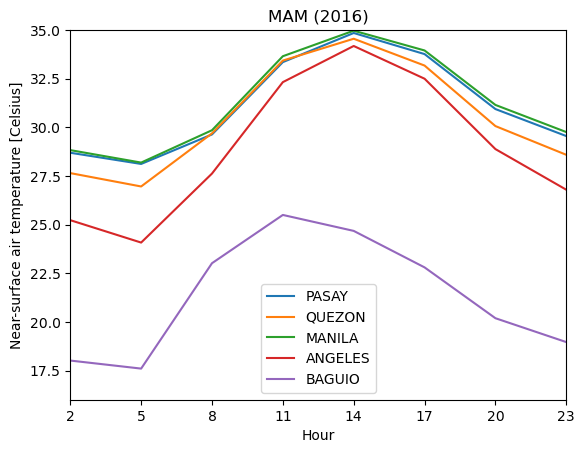
\includegraphics[width = 0.45 \textwidth]{hindcast/hourly-mean-mam}
			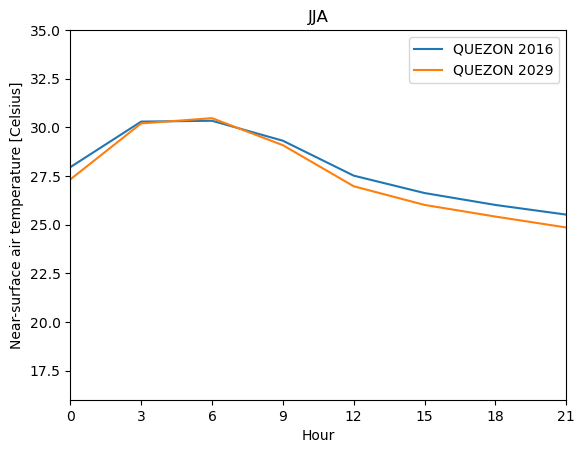
\includegraphics[width = 0.45 \textwidth]{hindcast/hourly-mean-jja}
			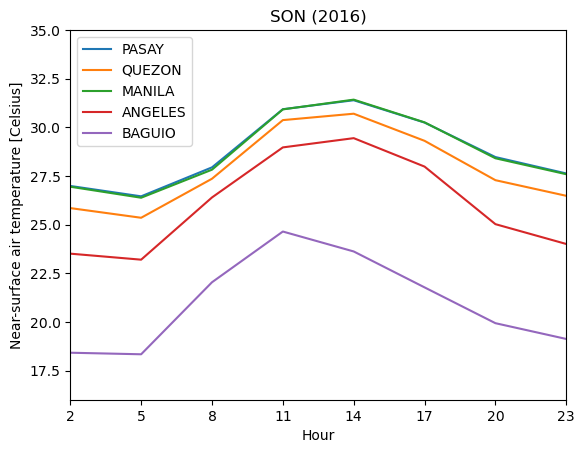
\includegraphics[width = 0.45 \textwidth]{hindcast/hourly-mean-son}
			\caption{
				Mean simulated near-surface air temperature each hour from 2015, December 1 to 2016, November 30, separated by three-month seasons (EIN15 ICBC with 8 km horizontal resolution).
				The seasons are:
					December, January, and February (DJF, upper left);
					March, April, and May (MAM, upper right);
					June, July, and August (JJA, lower left);
					and
					September, October, and November (SON, lower right).
			}
			\label{fig:hindcast-hourly-mean}
		\end{figure}
	
		Figure \ref{fig:hindcast-hourly-mean} shows the diurnal mean simulated near-surface air temperature from December 2015 to November 2016, split into three-month seasons:
			December, January, and February (DJF);
			March, April, and May (MAM);
			June, July, and August (JJA);
			and
			September, October, and November (SON).
		In all seasons, the mean air temperature is at its lowest at 9 PM, and peaks at 6 AM for all cities except Baguio, which peaks at 3 AM.
		The MAM season, corresponding to the Philippine's hot dry season, exhibits the highest air temperature compared to other seasons, in both daytime and nighttime.
		The JJA and SON seasons, which correspond to the Philippine wet season, show similar diurnal temperature patterns.
		The results for DJF, which correspond to the cool dry season, differ between cities.
		For the cities of Pasay, Quezon, and Manila, the DJF season has a similar pattern to JJA and SON.
		For the cities of Angeles and Baguio, the DJF season has cooler nighttime air temperature compared to JJA and SON, but have similar daytime air temperature.
		
		\begin{table}[]
			\caption{
				Mean simulated near-surface air temperature in degrees Celsius per season at 6 AM (Day), 6 PM (Night), and their difference (Diff.). Data simulated from December 2015 to November 2016.
			}
			\label{tab:hindcast-difference-day-night}
			\centering
			\begin{tabular}{lSSSSS}
				\hline \hline
				& {Pasay} & {Quezon} & {Manila} & {Angeles} & {Baguio} \\
				\hline
				      & \multicolumn{5}{c}{\textit{DJF}}           \\
				Day   & 32.0  & 31.6   & 32.2   & 30.5    & 23.4   \\
				Night & 27.2  & 25.8   & 27.1   & 22.9    & 16.7   \\
				Diff. & 4.8   & 5.8    & 5.1    & 7.6     & 6.7    \\
				& \multicolumn{5}{c}{\textit{MAM}}           \\
				Day   & 34.9  & 34.6   & 35.0   & 34.2    & 24.7   \\
				Night & 28.7  & 27.6   & 28.8   & 25.2    & 18.0   \\
				Diff. & 6.2   & 6.9    & 6.1    & 9.0     & 6.7    \\
				& \multicolumn{5}{c}{\textit{JJA}}           \\
				Day   & 31.3  & 30.3   & 31.1   & 29.7    & 22.8   \\
				Night & 27.3  & 26.0   & 27.3   & 24.2    & 19.1   \\
				Diff. & 3.9   & 4.3    & 3.8    & 5.4     & 3.7    \\
				& \multicolumn{5}{c}{\textit{SON}}           \\
				Day   & 31.4  & 30.7   & 31.4   & 29.4    & 23.6   \\
				Night & 27.0  & 25.9   & 26.9   & 23.5    & 18.4   \\
				Diff. & 4.4   & 4.9    & 4.5    & 5.9     & 5.2 \\
			  	\hline		
  			\end{tabular}
		\end{table}
		
		Table \ref{tab:hindcast-difference-day-night} shows the difference between daytime and noontime air temperature per season from December 2015 to November 2016.
		Since the diurnal air temperature peaks at 6 AM, this hour was chosen to represent daytime, while 6 PM is chosen to represent nighttime.
		The difference is greatest during the MAM season, and the least during JJA.
		Pasay and Manila have the least difference between day and night temperature,
			with a temperature of $\qty{3.9}{\degreeCelsius}$ and $\qty{3.8}{\degreeCelsius}$ during the JJA season,
			and a temperature of $\qty{6.2}{\degreeCelsius}$ and $\qty{6.1}{\degreeCelsius}$ during the MAM season,
			respectively.
		Meanwhile, Angeles shows the greatest difference, with a temperature of $\qty{5.4}{\degreeCelsius}$ during the JJA season, and $\qty{6.1}{\degreeCelsius}$ during the MAM season.
		These results may be explained by the relative urbanization of these cities.
		One characteristic of urban heat islands are high temperature at nighttime (\cite{Oke2017urban}).
		Pasay and Manila are the most urbanized among the cities, with little green spaces,
			and Quezon has relatively more green spaces compared to the other two cities (\cite{Bilang2022}).
		Furthermore, Angeles has vast green spaces surrounding it, which may explain the high difference between daytime and nighttime temperatures.
	
\section{Forecast}
	\subsection{SARIMA}
				
		\begin{figure}
			\centering
			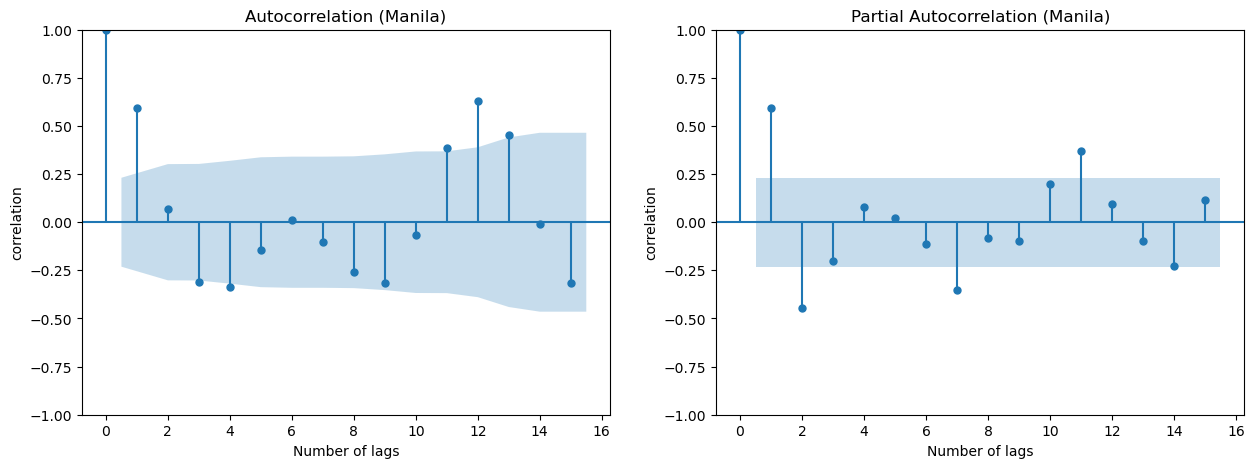
\includegraphics[width=\textwidth]{SARIMA/autocorrelations}
			\caption{
				Autocorrelation plots for the monthly mean time series data of Manila near-surface air temperature.
			}
			\label{fig:sarima-autocorrelations}
		\end{figure}	
		
		Figure \ref{fig:sarima-autocorrelations} shows the autocorrelation plots for Manila.
		For the autocorrelation plot, 
			there are significant negative correlations at $\num{3}$ and $\num4$ lags,
			suggesting that $p = 3$ and $p = 4$ are possible good values for the autoregressive factor.
		For the partial autocorrelation plot,
			there is a significant positive correlation at $\num{1}$ and $\num{2}$ lags,
			which suggest that $q = 1$ and $q = 2$ are possible good values for the moving average factor.
		
		\begin{table}[]
			\centering
			\caption{
				Evaluation results of various SARIMA parameters:
				Akaike information criterion (AIC),
				mean bias (MB),
				mean absolute error (MAE),
				and
				root mean square error (RMSE).
				Bolded parameters are best-performing out of all listed.
			}
			\label{tab:evaluation-sarima-parameters}
			\begin{tabular}{ccSSSS}
				\hline \hline
				{Order (p, d, q)} & {Seasonal Order (P, D, Q, S)} & {AIC}  & {MB}     & {MAE}   & {RMSE}  \\
				\hline
				(3, 1, 3)                           & None                                            & 126  & -0.938 & 1.00  & 1.24  \\
				(4, 1, 2)                           & None                                            & 130  & -0.217 & 0.800 & 1.07  \\
				(3, 1, 3)                           & (1, 1, 1, 12)                                   & 89.8 & -0.396 & 0.473 & 0.643 \\
				\textbf{(4, 1, 2)}                  & \textbf{(1, 1, 1, 12)}                          & 88.6 & -0.330 & 0.426 & 0.599 \\
				(3, 1, 3)                           & (1, 1, 0, 12)                                   & 89.5 & -0.383 & 0.520 & 0.680 \\
				(4, 1, 2)                           & (1, 1, 0, 12)                                   & 91.4 & -0.165 & 0.436 & 0.558 \\
				\hline			
			\end{tabular}
		\end{table}
	
		\begin{figure}
			\centering
			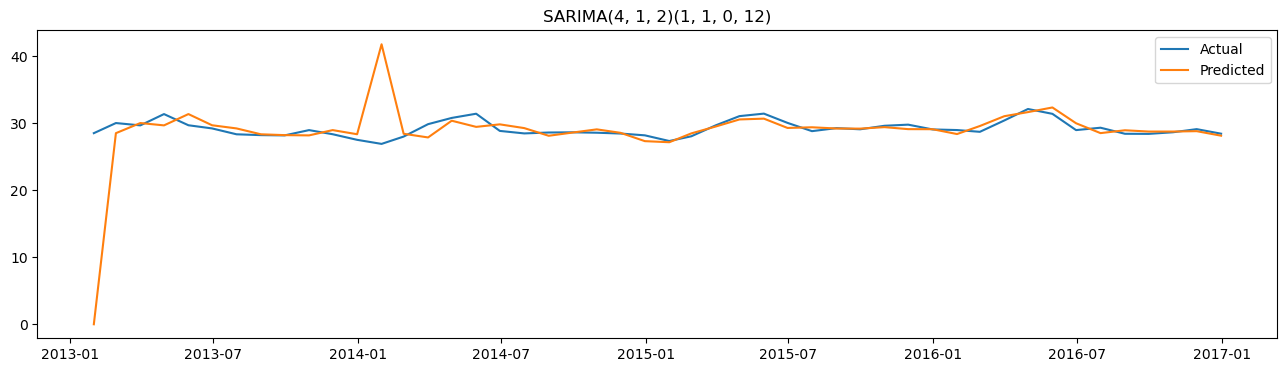
\includegraphics[width=\textwidth]{SARIMA/4 1 2 1 1 1 0 12 train}
			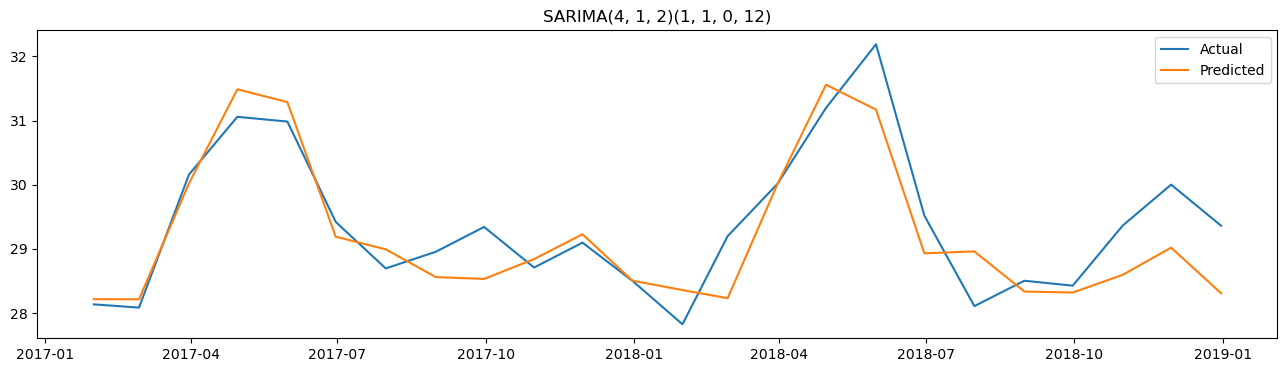
\includegraphics[width=\textwidth]{SARIMA/4 1 2 1 1 1 0 12 test}
			\caption{
				Graph of the best-performing model, $\operatorname{SARIMA}(4,1,2)(1,1,1,12)$, on training data (above) and testing data (below).
			}
			\label{fig:sarima-best-training-testing}
		\end{figure}
	
		Table \ref{tab:evaluation-sarima-parameters} shows the evaluation results of various SARIMA parameters.
		Models without a seasonal order show a higher AIC, MAE, and RMSE compared to models that do.
		Out of all tested models, the $\operatorname{SARIMA}(4,1,2)(1,1,1,12)$ model exhibits the least AIC, MAE, and RMSE values, which indicate that this is the best-performing model out of all the models tested. Figure \ref{fig:sarima-best-training-testing} shows a graph of this model over testing and training data.

\section{Limitations}
	One limitation of this study is that it only studies one variable, namely: near-surface air temperature.
	It does not examine ground temperature or temperature at different elevations.
	It also does not examine other factors that may be relevant to the study of urban heat islands, such as humidity, wind speed, wind direction, or precipitation. 
	Another limitation is that this study chose six specific cities to study: Angeles, Baguio, Manila, Olongapo, Pasay, and Quezon.
	Future studies may choose to study more cities.
	Another limitation is that this study only examines the three-year period from 2015 to 2017.
	Future studies may choose to study these other variables or study longer timeframes.
	
	There are many factors that can affect the findings. 
	Firstly, the physics schemes used in this run are all the default schemes, with the exception of the Community Land Model version 4.5 being chosen over the default BATS1e. 
	These runs do not use other models such as a lake model or a chemistry model, which may make the simulations more accurate and is an avenue for future research.
	Next, simulations are compared to the weather station data from the ISD.
	Only six stations were considered in this study.
	The data will be as accurate as the instruments used to record the data.
	Lastly, the study only used one domain.
	Changing the size and location of the domain without tweaking other settings can change the accuracy of the simulation.
	\stopcontents[chapters]
	\clearpage
	
\chapter{Conclusion}
	\Mprintcontents
	\label{ch:conclusion}
	\section{Conclusion}
	The general objective of the study was to forecast the effect of the urban heat island on near-surface air temperature in select highly-urbanized cities of Luzon, Philippines.
	The simulation used was RegCM5, a limited-area, long-term climate model developed by the International Center for Theoretical Physics.
	
	First, sensitivity runs were conducted and evaluated to determine the accuracy of RegCM5 in simulating near-surface air temperature in select cities of Luzon.
	The results show that in general, using a finer horizontal resolution increases the accuracy of a simulation.
	Using the EIN15 dataset for initial conditions and boundary conditions, together with an $\qty{8}{km}$ horizontal resolution shows the best results among all results tested, with an index of agreement ranging from $\numrange{0.78}{0.91}$.
	Furthermore, the mean bias, root mean square error, and mean absolute error for the run fall within the recommended values of $\leq \pm \qty{2.0}{\degreeCelsius}$, $\leq \qty{3.5}{\degreeCelsius}$, and $\leq \pm \qty{2.0}{\degreeCelsius}$ respectively.
	The CNRM-CM5 dataset for initial conditions and boundary conditions show an index of agreement of $\numrange{0.67}{0.81}$, indicating that a finer resolution maybe be needed in order to get accurate results when using this dataset.
	
	Second, a hindcast from 2013 to 2018, and a forecast from 2027-2031 was run and analysed.
	Results show that highly-urbanized cities exhibit a smaller difference between daytime and nighttime temperature compared to less urbanized ones.
	Pasay and Manila have the highest mean urban heat island intensity among the cities studied: 
		$\qty{1.75}{\degreeCelsius}$ and $\qty{1.72}{\degreeCelsius}$ from 2013 to 2018,
		and
		$\qty{1.82}{\degreeCelsius}$ and $\qty{1.85}{\degreeCelsius}$ from 2027-2031, respectively.
	Maximum urban heat island intensity can reach 
		$\qtyrange{4.1}{7.7}{\degreeCelsius}$ from 2013 to 2018,
		and
		$\qtyrange{4.2}{8.2}{\degreeCelsius}$ from 2027-2031.
	
	Third, a seasonal autoregressive integrated moving average (SARIMA) model used to forecast air temperature.
	Multiple sets of parameters were first tested and evaluated to see which parameters performed the best.
	The best-performing one was chosen to forecast data.
	SARIMA forecasts mean near-surface air temperature of cities to increase by $\qtyrange{0.9}{1.0}{\degreeCelsius}$ by 2030.

The study overall shows that RegCM5 can be accurate in simulating urban heat, but can be improved with finer resolution and coupling with other models, and that 
the urban heat island effect will be greater by 2030.
	
\section{Recommendations}
	For researchers, possible avenues for future research include:
	incorporating other physics models, using different datasets for initial conditions and boundary conditions, using different studying other cities in the Philippines, and using finer horizontal resolutions and longer time scales.
	Researchers may also incorporate more sophisticated modeling of anthropogenic heat into RegCM.
	For city planners and local government officials, these results can be used to better study heat in cities, implement policies and projects to reduce heat in cities, as well as to improve disaster and risk reduction management.
	\stopcontents[chapters]
	\clearpage

%%%%%%%%%%%%%%%%%%%%%%%%%%%%%%%%%%%%%%%
% BIBLIOGRAPHY

%\nocite{*}
\printbibliography

\clearpage

\appendix
\chapter{Budget and Timeline}
	\label{app:budget-timeline}
	Table \ref{tab:budget} shows the budget for this study.
The meteorological data for the initial and boundary conditions as well as the simulation model are both free.
They are available to download on the internet.
The PC Workstation is available in the laboratory.
Printing and bookbinding is estimated to be 500 Philippine Pesos,
and will be the only cost for the study.

\begin{table}
	\caption{Budget for this study.}
	\label{tab:budget}
	\centering
	\begin{tabular}{l r}
		\hline \hline
		Item & Price (PHP) \\
		\hline
		Meteorological data	& 0 \\
		RegCM & 0 \\
		PC Workstation & 0 \\
		Printing and bookbinding & 500 \\
		\hline
		\textbf{Total} & \textbf{500} \\
		\hline
	\end{tabular}
\end{table}

Figure \ref{fig:timeline} shows the timeline for this study.
Term 1 of Academic Year 2024-2025 will be dedicated to the proposal of the study and the preparation to run the simulations.
The proposal of this study is expected to be conducted by October.
After the proposal, meteorological data for the initial and boundary conditions for the data will be downloaded.
With the large file size, it is expected to take a while to download it.
Term 2 of Academic Year 2024-2025 will be dedicated to the running of simulations and the analysis of the results.
Term 3 of Academic Year 2024-2025 will be dedicated to finishing the manuscript and defending the study.

\begin{figure}
	\centering
	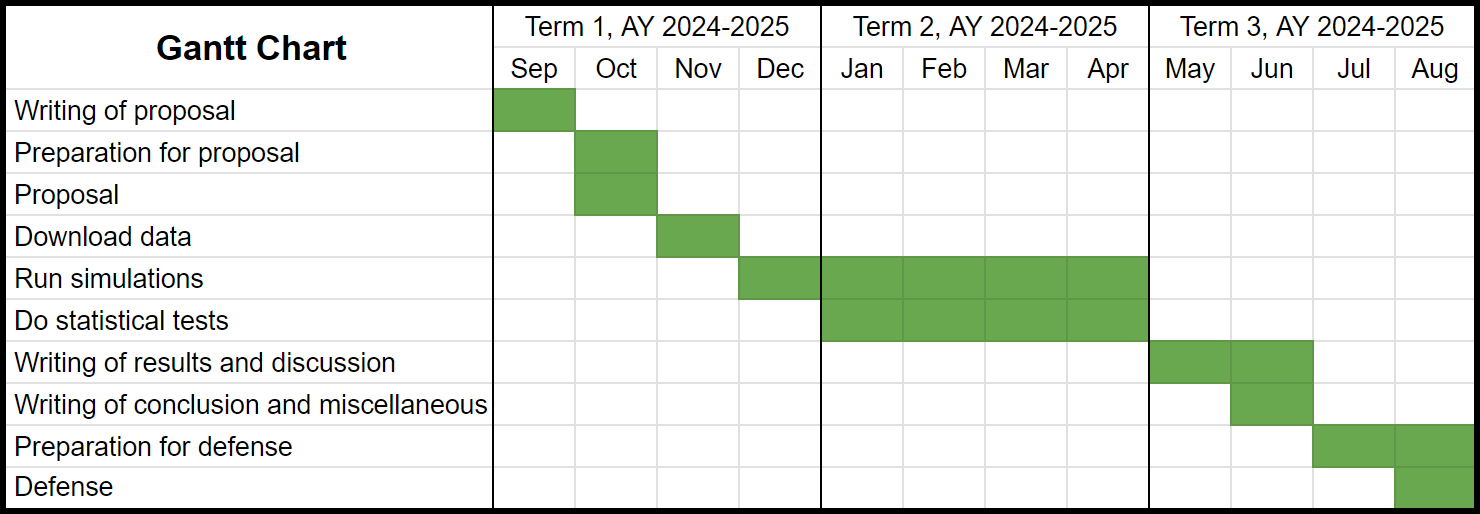
\includegraphics[width=\textwidth]{proposal-gantt-chart}
	\caption{Timeline for this study.}
	\label{fig:timeline}
\end{figure}
	
\chapter{Model Evaluation Graphs}
	\label{app:model-evaluation-graphs}
	\begin{figure}	
	\centering
	\includegraphics[width = 0.8 \textwidth]{EIN15 16 km/Angeles}
	\includegraphics[width = 0.8 \textwidth]{EIN15 8 km/Angeles}
	\includegraphics[width = 0.8 \textwidth]{CNRM 16 km/Angeles}
	\includegraphics[width = 0.8 \textwidth]{CNRM 8 km/Angeles}
	\caption{
		A comparison of the simulated data (orange) and observed data (blue) in the city of Angeles for each of the four sensitivity runs.
	}
	\label{fig:appendix-sim-vs-observed-angeles}
\end{figure}

\begin{figure}	
	\centering
	\includegraphics[width = 0.8 \textwidth]{EIN15 16 km/Baguio}
	\includegraphics[width = 0.8 \textwidth]{EIN15 8 km/Baguio}
	\includegraphics[width = 0.8 \textwidth]{CNRM 16 km/Baguio}
	\includegraphics[width = 0.8 \textwidth]{CNRM 8 km/Baguio}
	\caption{
		A comparison of the simulated data (orange) and observed data (blue) in the city of Baguio for each of the four sensitivity runs.
	}
	\label{fig:appendix-sim-vs-observed-baguio}
\end{figure}

\begin{figure}	
	\centering
	\includegraphics[width = 0.8 \textwidth]{EIN15 16 km/Manila}
	\includegraphics[width = 0.8 \textwidth]{EIN15 8 km/Manila}
	\includegraphics[width = 0.8 \textwidth]{CNRM 16 km/Manila}
	\includegraphics[width = 0.8 \textwidth]{CNRM 8 km/Manila}
	\caption{
		A comparison of the simulated data (orange) and observed data (blue) in the city of Manila for each of the four sensitivity runs.
	}
	\label{fig:appendix-sim-vs-observed-manila}
\end{figure}

\begin{figure}	
	\centering
	\includegraphics[width = 0.8 \textwidth]{EIN15 16 km/Olongapo}
	\includegraphics[width = 0.8 \textwidth]{EIN15 8 km/Olongapo}
	\includegraphics[width = 0.8 \textwidth]{CNRM 16 km/Olongapo}
	\includegraphics[width = 0.8 \textwidth]{CNRM 8 km/Olongapo}
	\caption{
		A comparison of the simulated data (orange) and observed data (blue) in the city of Olongapo for each of the four sensitivity runs.
	}
	\label{fig:appendix-sim-vs-observed-olongapo}
\end{figure}

\begin{figure}	
	\centering
	\includegraphics[width = 0.8 \textwidth]{EIN15 16 km/Pasay}
	\includegraphics[width = 0.8 \textwidth]{EIN15 8 km/Pasay}
	\includegraphics[width = 0.8 \textwidth]{CNRM 16 km/Pasay}
	\includegraphics[width = 0.8 \textwidth]{CNRM 8 km/Pasay}
	\caption{
		A comparison of the simulated data (orange) and observed data (blue) in the city of Pasay for each of the four sensitivity runs.
	}
	\label{fig:appendix-sim-vs-observed-pasay}
\end{figure}

\begin{figure}	
	\centering
	\includegraphics[width = 0.8 \textwidth]{EIN15 16 km/Quezon}
	\includegraphics[width = 0.8 \textwidth]{EIN15 8 km/Quezon}
	\includegraphics[width = 0.8 \textwidth]{CNRM 16 km/Quezon}
	\includegraphics[width = 0.8 \textwidth]{CNRM 8 km/Quezon}
	\caption{
		A comparison of the simulated data (orange) and observed data (blue) in the city of Quezon for each of the four sensitivity runs.
	}
	\label{fig:appendix-sim-vs-observed-quezon}
\end{figure}
	
\chapter{Installing, Testing, and Running RegCM}
	\label{app:regcm-install-run}
	This appendix chapter will briefly discuss how to install, test, and run RegCM.
This chapter will also discuss how to access the User's Guide for RegCM.
Most of the instructions are already covered in the User's Guide,
	but the other parts that were not covered will be discussed here.

\section{Prerequisites}
	Since RegCM is a GNU-based system, a familiarity on how to use the Linux command line is a must.
	Also, since RegCM is written in Fortran, you need a Fortran compiler.
	
	The model needs at least two libraries:
	\begin{itemize}
		\item A netCDF Library 
		(\url{https://www.unidata.ucar.edu/software/netcdf/}),
		which you can test if it's installed by doing
		\texttt{nf-config --version},
		and
		\item MPI MPI Library
		(\url{http://www.openmpi.org/}),
		which you can test if it's installed by doing
		\texttt{ompi\_info --version ompi release}
	\end{itemize}
	The software is already installed on the desktops from Ubuntu
	repositories. You can find a script in the \texttt{Tools/Script} directory
	to compile required library from source.
	
	More on prerequisites are found in Section 3.1 and 3.2 of the User's Guide.
	
\section{Obtaining the Model and Documentation}
	According to the User's Guide, the packed archive file with the model code can be downloaded from the G-forge website: 
		\url{http://gforge.ictp.it/gf/project/regcm/frs}.
	However, I could not access the site myself.
	Instead, I had to go into the model's GitHub site:
	\begin{center}
		\url{https://github.com/ICTP/RegCM}
	\end{center}
	to download it.
	From the GitHub website, under ``Releases'', there will be a release entitled ``NH V5 code''.
	Click on that, and you will see a link to download either a \texttt{zip} package or a \texttt{tar.gz} package.
	Download the \texttt{tar.gz} package, and extract the files from those packages using
	\begin{center}
		\texttt{tar -zxvf RegCM-5.0.0.tar.gz}.
	\end{center}
	Alternatively, if your machine has \texttt{git} and you want the most updated version of RegCM, you can use \texttt{git pull} to download the source code directly from the most recent commit to the GitHub master branch.
	Do note though, that the source code from the Releases tab may be different from the most recent commits to the master branch.

\section{Accessing the User's Guide}
	Before doing this section, do a quick Google search or check the lab's files (NAS or Google Drive) to see if an updated version of the RegCM User's Guide is available online.
	If there is, then you don't need to compile the User's Guide yourself.

	The User's Guide does not come as a \texttt{pdf}.
	Instead, the User's Guide comes with the RegCM source code as \LaTeX\ code.
	You will need a \LaTeX\ distribution and compile the code yourself.
	I will not discuss how to install \LaTeX\ here, but this guide in StackExchange may be helpful to you:
	\begin{center}
		\url{https://stackoverflow.com/a/1017170}.
	\end{center}

	In the source code for RegCM, there is a folder called \texttt{Doc}.
	In that folder is the \LaTeX\ source code for the User's Guide, Developer Guide, and Reference Manual, and a commented version of the input file for RegCM.
	Use your \LaTeX\ distribution to compile the \texttt{UserGuide.tex} file under the \texttt{UserGuide} folder into a readable \texttt{pdf}.
	Following the User's Guide will be very helpful for setting up, testing, and running RegCM.
	
\section{Installing and Testing RegCM}
	from the RegCM root folder, you'll want to run the provided \texttt{configure} script by typing
	\begin{center}
		\texttt{./configure}
	\end{center}
	If you plan on using the Community Land Model 4.5 instead of the default Biosphere-Atmosphere Transfer Scheme, then you'll need to do 
	\begin{center}
		\texttt{./configure --enable-clm45}
	\end{center}
	instead.
	Then, you'll want to run
	\begin{center}
		\texttt{make install}
	\end{center}
	to install the software.
	For more detailed instructions, see Chapter 3 of the User's Guide.

\section{Downloading Global Datasets}
	Besides the time it takes to run RegCM itself, this step will take the most of your time.
	You will need various global datasets for RegCM's inputs.
	They can be found in
	\begin{center}
		\url{http://clima-dods.ictp.it/regcm4/}
	\end{center}
	and can be downloaded in the command line using either \texttt{curl} or \texttt{wget}.
	For example, to recursively download all files in a particular folder, you can use the \texttt{-r} and \texttt{-np} options for \texttt{wget} (which correspond to ``recursive'' and ``no parent'', respectively). 
	Also, it's VERY important to test if the files have downloaded properly, since sometimes the files may have been incompletely downloaded or have been corrupted.
	To do this, you can check with the \texttt{-c} option (which corresponds to ``continue'').
	Lastly, web crawlers are disallowed on the website for some bizzare reason!? So you'll need the \texttt{-e robots=off} option. 
	All in all, your download command might look like:
	\begin{center}
		\texttt{wget -c -r -np -e robots=off <url>}
	\end{center}
	Instead of recursion, you may also create a for loop to loop through multiple files.
	
	The datasets are BIG in size, and you may need to fill up about $\qty{100}{GB}$ of storage, maybe even more.
	Which datasets to download is up to your needs.
	For the datasets needed to test the model, please see Chapter 4 of the User's Guide.
	
\section{Running a Test Simulation}
	Running a test simulation using the model is covered in detail in Chapter 5 of the User's Guide, and will not be covered here.
	
	If you are using the CLM4.5 version of RegCM, then instead of the 
	\texttt{terrain}, \texttt{sst}, \texttt{icbc}, and \texttt{regcmMPI} programs,
	they will be replaced with 
	\texttt{terrainCLM45}, \texttt{sstCLM45}, \texttt{icbcCLM45}, and \texttt{regcmMPICLM45} programs.
	Furthermore, you will also need to run the \texttt{mksurfCLM45} program after running the \texttt{terrainCLM45} program.
	A summary of the inputs and outputs of RegCM are seen in the included schematic.
	\begin{figure}	
		\centering
		\includegraphics[width = \textwidth]{schematic-regcm-inputs-outputs}
		\caption{
			Schematic of the inputs and outputs of RegCM5 (with CLM 4.5)
		}
	\end{figure}
	
\section{Changing Settings and Running Your Own Simulations}
	RegCM parameters are covered in Chapter 6 of the User's Guide, and will not be covered here.
	Running your own simulation will be similar to running the test simulation, but now you have free reign to change parameters to fit your experiments.
	
	RegCM can be very computationally intensive, especially if you use a high number of CPU cores (and your machine might crash! It has happened to me multiple times).
	So you can run chunks of the simulation at a time using the 
	\texttt{\&restartparam} section, where \texttt{ifrest = .false.} indicates a first run, and \texttt{ifrest = .true.} indicates subsequent runs.
	When continuing a run:
		First set \texttt{ifrest} to \texttt{.true.},
		set \texttt{mdate1} to the value in \texttt{mdate2},
		and then
		define the new value for \texttt{mdate2}.
	I recommend doing small time intervals at a time (try one month first), then doing larger time intervals (two months, then three, \dots) to see how well your machine can handle RegCM.
	
	A good chosen \texttt{dt} is important, as a value too big will make the simulation stop, but a value too small will make the simulation take forever.
	As a rule of thumb, try a \texttt{dt} value not greater than three times the \text{ds} value.
	If the simulation tells you to use a lower value, then decrease it and rerun the simulation.
	
\section{Final Tips}
	Most of your time will be spent on waiting\dots\ and waiting\dots\ and waiting\dots.
	So be sure to plan your downloads/runs accordingly.
	Make sure that the datasets are properly downloaded and not incomplete/corrupted.
	Make sure to regularly check on your simulations to see if they are still running.
	Have an external drive handy so you can transfer the big output file from the machine when it's done.
	You can have multiple machines downloading datasets and then just transfer them to other machines as needed.
	Good luck!

\backmatter
\chapter{Colophon}
	This manuscript was typeset by the author using \LaTeX\  and the \texttt{memoir} class.
The \LaTeX\ typesetting system was created by Leslie Lamport.
The \TeX\ software, which forms the base for \LaTeX, was written by Donald Knuth.
The \texttt{memoir} class was created by Peter R. Wilson and Lars Madsen.

The file used to typeset this manuscript is a modified version of \texttt{DLSUdtp}, a \LaTeX\  document format for authors of De La Salle University (DLSU) dissertations, theses, proposals, or projects.
It was created by Dr. Lawrence Materum of the DLSU Department of Electronics and Communications Engineering.
It may be accessed on GitHub (https://github.com/melvincabatuan/ThesisLaTeXTemplate).
It is distributed under the LaTeX Project Public License (LPPL) (http://www.latex-project.org/lppl.txt) version 1.3, and may be used, distributed, and modified. 



\end{document}